%% HarvestMem 中文稿（v1.0 草稿）。编译：./build.sh
%% 数值一律通过 \V{键名} 从 data/values.yaml 读取：真实结果正常显示，理想示意值显示为红色，待确认信息显示为橙色方括号。
%% 投稿前：所有 ideal/todo 项替换为实测并改为 real，再把 \shownotestrue 改为 \shownotesfalse 去掉写作附录。
\documentclass[zihao=5,a4paper,UTF8,fontset=fandol]{ctexart}

\usepackage[top=2.4cm,bottom=2.4cm,left=2.3cm,right=2.3cm]{geometry}
\usepackage{amsmath,amssymb,bm}
\usepackage{graphicx}
\usepackage{booktabs,multirow,array,longtable,threeparttable}
\usepackage[table]{xcolor}
\usepackage[font=small,labelfont=bf,labelsep=quad,skip=4pt]{caption}
\usepackage{subcaption}
\usepackage{algorithm,algpseudocode}
\usepackage{enumitem}
\usepackage{tikz}
\usetikzlibrary{positioning,arrows.meta,shapes.geometric,shapes.misc,fit,backgrounds,calc,decorations.pathreplacing}
\usepackage[framemethod=TikZ]{mdframed}
\usepackage{amsthm}
\usepackage{pifont}
\usepackage{gbt7714}
\usepackage[colorlinks=true,linkcolor=blue!50!black,citecolor=blue!50!black,urlcolor=blue!50!black]{hyperref}

\graphicspath{{figures/}}
\linespread{1.32}
\setlength{\parskip}{0.2em}
\setlist{nosep,leftmargin=2.2em}
\ctexset{
  section={format=\large\bfseries\heiti,name={,},number=\arabic{section},aftername=\quad,beforeskip=1.1em,afterskip=0.6em},
  subsection={format=\normalsize\bfseries\heiti,beforeskip=0.8em,afterskip=0.4em},
  subsubsection={format=\normalsize\heiti,beforeskip=0.5em,afterskip=0.3em},
  abstractname={摘\quad 要}
}
\floatname{algorithm}{算法}
\renewcommand{\algorithmicrequire}{\textbf{输入：}}
\renewcommand{\algorithmicensure}{\textbf{输出：}}
\renewcommand{\topfraction}{0.9}
\renewcommand{\bottomfraction}{0.8}
\renewcommand{\textfraction}{0.08}
\renewcommand{\floatpagefraction}{0.85}
\setlength{\textfloatsep}{10pt plus 2pt minus 2pt}

%% ---------------- 数值宏
\newif\ifshownotes \shownotestrue
\theoremstyle{definition}
\newtheorem{proposition}{命题}
\newtheorem{definition}{定义}
\makeatletter
\newcommand{\defval}[3]{\expandafter\def\csname val@#1\endcsname{\csname fmt@#2\endcsname{#3}}}
\expandafter\def\csname fmt@real\endcsname#1{#1}
\expandafter\def\csname fmt@ideal\endcsname#1{\textcolor{red}{#1}}
\expandafter\def\csname fmt@todo\endcsname#1{\textcolor{orange!85!black}{[#1]}}
\newcommand{\V}[1]{\ifcsname val@#1\endcsname\csname val@#1\endcsname\else\textbf{\textcolor{magenta}{??#1}}\PackageWarning{values}{Undefined value #1}\fi}
\makeatother
% generated by tools/gen_values.py from data/values.yaml; do not edit
\defval{author1}{todo}{作者一}
\defval{author2}{todo}{作者二}
\defval{author3}{todo}{通信作者}
\defval{affil}{todo}{单位，城市 邮编}
\defval{email}{todo}{email@example.com}
\defval{fund}{todo}{基金项目名称（编号）}
\defval{n_dec}{real}{5318}
\defval{n_pairs}{real}{7841}
\defval{cov_u16}{real}{57.0}
\defval{cov_u16_miss}{real}{43.0}
\defval{cov_rand}{real}{43.2}
\defval{cov_recent}{real}{8.0}
\defval{cov_k4}{real}{87.6}
\defval{cov_k8}{real}{99.6}
\defval{cov_k4_b8}{real}{85.9}
\defval{cov_u32}{real}{88.3}
\defval{cnt_u16}{real}{43.1}
\defval{cnt_k8}{real}{99.2}
\defval{last_u16}{real}{67.5}
\defval{gap_u}{real}{14}
\defval{gap_k8}{real}{17}
\defval{near_u}{real}{4.2}
\defval{theory_err}{real}{0.012}
\defval{cov_u_early}{real}{97.8}
\defval{cov_u_late}{real}{26.4}
\defval{last_u_late}{real}{21.7}
\defval{cov_k8_late}{real}{94.6}
\defval{pick_frames}{real}{12}
\defval{near_frac}{real}{5}
\defval{occl_invis}{real}{78}
\defval{evt_f1_plateau}{real}{1.000}
\defval{spec_white}{real}{1.5}
\defval{spec_white_f1}{real}{0.987}
\defval{spec_ou_f1}{real}{0.953}
\defval{white1_plain_f1}{real}{0.846}
\defval{white1_plain_cnt}{real}{37}
\defval{white1_hyst_f1}{real}{0.999}
\defval{fdm_loc}{real}{0.48}
\defval{fdm_dist}{real}{0.34}
\defval{fdm_anchor_rec}{real}{99.8}
\defval{fdm_postgust_rec}{real}{78.3}
\defval{fdm_hidden_pre}{real}{138/138}
\defval{fdm_hidden_post}{real}{0/138}
\defval{perframe_cnt}{real}{62}
\defval{hsv_light_f1}{real}{0.1}
\defval{samgt_light_f1}{real}{0.999}
\defval{sam_ms_b}{real}{94}
\defval{sam_ms_h}{real}{309}
\defval{pekm_us}{real}{117}
\defval{unif_us}{real}{39}
\defval{robomme_nomem_a}{real}{66.7}
\defval{robomme_nomem_b}{real}{1.7}
\defval{robomme_half_a}{real}{64.4}
\defval{robomme_half_b}{real}{26.7}
\defval{ll_succ_a}{real}{5}
\defval{ll_succ_b}{real}{51}
\defval{ll_first_a}{real}{25}
\defval{ll_first_b}{real}{76}
\defval{ll_wrist_a}{real}{60}
\defval{ll_wrist_b}{real}{0}
\defval{ll_resume_a}{real}{214}
\defval{ll_resume_b}{real}{16}
\defval{v1_n}{real}{150}
\defval{v1_cnt_k0}{real}{67.3}
\defval{v1_cnt_k4}{real}{62.0}
\defval{v1_cnt_k8}{real}{70.7}
\defval{v1_occ_k0}{real}{30.0}
\defval{v1_occ_k4}{real}{29.3}
\defval{v1_occ_k8}{real}{31.3}
\defval{v1_holm}{real}{1.00}
\defval{v1_cnt_memfail}{real}{0}
\defval{v1_occ_wrong_k0}{real}{8.0}
\defval{v1_occ_wrong_k4}{real}{14.0}
\defval{v1_occ_wrong_k8}{real}{13.3}
\defval{v1_frame0}{real}{100}
\defval{v1_leaf_lift}{real}{94.5}
\defval{v1_hidden_ripe_frac}{real}{73}
\defval{v1_nopregust_a}{real}{32.5}
\defval{v1_nopregust_b}{real}{25.0}
\defval{budget_B}{real}{16}
\defval{exec_h}{real}{16}
\defval{radius_r}{real}{3}
\defval{tol}{real}{5}
\defval{train_steps}{real}{12000}
\defval{n_val}{real}{150}
\defval{audit_n}{real}{50}
\defval{aud_cnt_o1}{ideal}{14}
\defval{aud_cnt_o2}{ideal}{18}
\defval{aud_cnt_o3}{ideal}{96}
\defval{aud_occ_o1}{ideal}{26}
\defval{aud_occ_o2}{ideal}{94}
\defval{aud_occ_o3}{ideal}{96}
\defval{exp_cnt}{ideal}{93.5}
\defval{exp_occ}{ideal}{95.0}
\defval{clip_cnt}{ideal}{0.21}
\defval{clip_occ}{ideal}{0.18}
\defval{demo_n}{real}{200}
\defval{det_n_ep}{ideal}{300}
\defval{det_n_ev}{ideal}{812}
\defval{det_n_fail}{ideal}{164}
\defval{det_geo_p}{ideal}{0.832}
\defval{det_geo_r}{ideal}{1.000}
\defval{det_geo_f1}{ideal}{0.908}
\defval{det_geo_cnt}{ideal}{61.3}
\defval{det_geo_fp}{ideal}{100}
\defval{det_geo_light}{ideal}{1.000}
\defval{det_fdm_p}{ideal}{0.903}
\defval{det_fdm_r}{ideal}{0.981}
\defval{det_fdm_f1}{ideal}{0.940}
\defval{det_fdm_cnt}{ideal}{74.7}
\defval{det_fdm_fp}{ideal}{38}
\defval{det_fdm_light}{ideal}{0.214}
\defval{det_grip_p}{ideal}{0.887}
\defval{det_grip_r}{ideal}{0.952}
\defval{det_grip_f1}{ideal}{0.918}
\defval{det_grip_cnt}{ideal}{66.0}
\defval{det_grip_fp}{ideal}{41}
\defval{det_grip_light}{ideal}{0.918}
\defval{det_pv_p}{ideal}{0.942}
\defval{det_pv_r}{ideal}{0.957}
\defval{det_pv_f1}{ideal}{0.949}
\defval{det_pv_cnt}{ideal}{81.3}
\defval{det_pv_fp}{ideal}{12}
\defval{det_pv_light}{ideal}{0.902}
\defval{det_pp_p}{ideal}{0.901}
\defval{det_pp_r}{ideal}{0.963}
\defval{det_pp_f1}{ideal}{0.931}
\defval{det_pp_cnt}{ideal}{72.0}
\defval{det_pp_fp}{ideal}{33}
\defval{det_pp_light}{ideal}{0.931}
\defval{det_pe_p}{ideal}{0.978}
\defval{det_pe_r}{ideal}{0.983}
\defval{det_pe_f1}{ideal}{0.980}
\defval{det_pe_cnt}{ideal}{92.7}
\defval{det_pe_fp}{ideal}{4}
\defval{det_pe_light}{ideal}{0.962}
\defval{det_pe_tc}{ideal}{1}
\defval{det_pe_tr}{ideal}{0}
\defval{det_pe_tr90}{ideal}{2}
\defval{det_pe_kf}{ideal}{0.987}
\defval{pedet_params}{ideal}{1.9}
\defval{pedet_ms}{ideal}{1.6}
\defval{fig_light_x.1}{real}{0.5}
\defval{fig_light_x.2}{real}{0.7}
\defval{fig_light_x.3}{real}{1.0}
\defval{fig_light_x.4}{real}{1.3}
\defval{fig_light_x.5}{real}{1.6}
\defval{fig_light_x}{real}{0.5, 0.7, 1.0, 1.3, 1.6}
\defval{fig_light_pedet.1}{ideal}{0.951}
\defval{fig_light_pedet.2}{ideal}{0.972}
\defval{fig_light_pedet.3}{ideal}{0.98}
\defval{fig_light_pedet.4}{ideal}{0.975}
\defval{fig_light_pedet.5}{ideal}{0.958}
\defval{fig_light_pedet}{ideal}{0.951, 0.972, 0.98, 0.975, 0.958}
\defval{fig_light_fdm.1}{ideal}{0.12}
\defval{fig_light_fdm.2}{ideal}{0.48}
\defval{fig_light_fdm.3}{ideal}{0.94}
\defval{fig_light_fdm.4}{ideal}{0.61}
\defval{fig_light_fdm.5}{ideal}{0.15}
\defval{fig_light_fdm}{ideal}{0.12, 0.48, 0.94, 0.61, 0.15}
\defval{fig_light_grip.1}{ideal}{0.918}
\defval{fig_light_grip.2}{ideal}{0.918}
\defval{fig_light_grip.3}{ideal}{0.918}
\defval{fig_light_grip.4}{ideal}{0.918}
\defval{fig_light_grip.5}{ideal}{0.918}
\defval{fig_light_grip}{ideal}{0.918, 0.918, 0.918, 0.918, 0.918}
\defval{hem_mw}{real}{2}
\defval{hem_c}{real}{4}
\defval{hem_smax}{real}{3}
\defval{cap_hem}{real}{14}
\defval{cap_k8}{real}{4.3}
\defval{cap_u}{real}{1.0}
\defval{cap_flat_max}{real}{7}
\defval{hem_params}{ideal}{0.14}
\defval{hem_ms}{ideal}{0.21}
\defval{fm_steps}{todo}{10}
\defval{c_k0.1}{ideal}{58}
\defval{c_k0.2}{ideal}{45}
\defval{c_k0.3}{ideal}{22}
\defval{c_k0.4}{ideal}{9}
\defval{c_k0.5}{ideal}{16}
\defval{c_k0}{ideal}{58, 45, 22, 9, 16}
\defval{c_k4.1}{ideal}{78}
\defval{c_k4.2}{ideal}{30}
\defval{c_k4.3}{ideal}{16}
\defval{c_k4.4}{ideal}{10}
\defval{c_k4.5}{ideal}{16}
\defval{c_k4}{ideal}{78, 30, 16, 10, 16}
\defval{c_k8.1}{ideal}{88}
\defval{c_k8.2}{ideal}{20}
\defval{c_k8.3}{ideal}{12}
\defval{c_k8.4}{ideal}{10}
\defval{c_k8.5}{ideal}{20}
\defval{c_k8}{ideal}{88, 20, 12, 10, 20}
\defval{c_hem.1}{ideal}{96}
\defval{c_hem.2}{ideal}{14}
\defval{c_hem.3}{ideal}{10}
\defval{c_hem.4}{ideal}{10}
\defval{c_hem.5}{ideal}{20}
\defval{c_hem}{ideal}{96, 14, 10, 10, 20}
\defval{c_k0_s}{ideal}{38.7}
\defval{c_k4_s}{ideal}{52.0}
\defval{c_k8_s}{ideal}{58.7}
\defval{c_hem_s}{ideal}{64.0}
\defval{c_k0_mem}{ideal}{44.7}
\defval{c_k4_mem}{ideal}{30.7}
\defval{c_k8_mem}{ideal}{21.3}
\defval{c_hem_mem}{ideal}{16.0}
\defval{c_k0_op}{ideal}{16.7}
\defval{c_k4_op}{ideal}{17.3}
\defval{c_k8_op}{ideal}{20.0}
\defval{c_hem_op}{ideal}{20.0}
\defval{c_k0_err}{ideal}{0.52}
\defval{c_k8_err}{ideal}{0.23}
\defval{c_hem_err}{ideal}{0.17}
\defval{c_k4_err}{ideal}{0.34}
\defval{c_d4}{ideal}{+13.3}
\defval{c_d4_ci}{ideal}{[4.7, 22.0]}
\defval{c_d8}{ideal}{+20.0}
\defval{c_d8_ci}{ideal}{[11.3, 28.7]}
\defval{c_dh}{ideal}{+25.3}
\defval{c_dh_ci}{ideal}{[16.7, 34.0]}
\defval{c_dh_p}{ideal}{$<$0.001}
\defval{c_dh8}{ideal}{+5.3}
\defval{c_dh8_ci}{ideal}{[$-$1.3, 12.0]}
\defval{c_dh_noguard}{ideal}{+22.7}
\defval{c_dh_noguard_ci}{ideal}{[12.0, 33.3]}
\defval{c_clip}{ideal}{22.1}
\defval{cN_k0.1}{ideal}{56.3}
\defval{cN_k0.2}{ideal}{37.3}
\defval{cN_k0.3}{ideal}{23.5}
\defval{cN_k0}{ideal}{56.3, 37.3, 23.5}
\defval{cN_k8.1}{ideal}{68.8}
\defval{cN_k8.2}{ideal}{58.8}
\defval{cN_k8.3}{ideal}{49.0}
\defval{cN_k8}{ideal}{68.8, 58.8, 49.0}
\defval{cN_hem.1}{ideal}{70.8}
\defval{cN_hem.2}{ideal}{62.7}
\defval{cN_hem.3}{ideal}{58.8}
\defval{cN_hem}{ideal}{70.8, 62.7, 58.8}
\defval{cN_gain_h0.1}{ideal}{+14.5}
\defval{cN_gain_h0.2}{ideal}{+25.4}
\defval{cN_gain_h0.3}{ideal}{+35.3}
\defval{cN_gain_h0}{ideal}{+14.5, +25.4, +35.3}
\defval{cN_gain_h8.1}{ideal}{+2.0}
\defval{cN_gain_h8.2}{ideal}{+3.9}
\defval{cN_gain_h8.3}{ideal}{+9.8}
\defval{cN_gain_h8}{ideal}{+2.0, +3.9, +9.8}
\defval{o_k0.1}{ideal}{92}
\defval{o_k0.2}{ideal}{22}
\defval{o_k0.3}{ideal}{14}
\defval{o_k0.4}{ideal}{8}
\defval{o_k0.5}{ideal}{14}
\defval{o_k0}{ideal}{92, 22, 14, 8, 14}
\defval{o_k4.1}{ideal}{94}
\defval{o_k4.2}{ideal}{20}
\defval{o_k4.3}{ideal}{13}
\defval{o_k4.4}{ideal}{9}
\defval{o_k4.5}{ideal}{14}
\defval{o_k4}{ideal}{94, 20, 13, 9, 14}
\defval{o_k8.1}{ideal}{91}
\defval{o_k8.2}{ideal}{21}
\defval{o_k8.3}{ideal}{14}
\defval{o_k8.4}{ideal}{9}
\defval{o_k8.5}{ideal}{15}
\defval{o_k8}{ideal}{91, 21, 14, 9, 15}
\defval{o_hem.1}{ideal}{93}
\defval{o_hem.2}{ideal}{21}
\defval{o_hem.3}{ideal}{13}
\defval{o_hem.4}{ideal}{9}
\defval{o_hem.5}{ideal}{14}
\defval{o_hem}{ideal}{93, 21, 13, 9, 14}
\defval{o_k0_s}{ideal}{61.3}
\defval{o_k4_s}{ideal}{62.7}
\defval{o_k8_s}{ideal}{60.7}
\defval{o_hem_s}{ideal}{62.0}
\defval{o_k0_mem}{ideal}{24.0}
\defval{o_k4_mem}{ideal}{22.0}
\defval{o_k8_mem}{ideal}{23.3}
\defval{o_hem_mem}{ideal}{22.7}
\defval{o_d4}{ideal}{+1.3}
\defval{o_d4_ci}{ideal}{[$-$6.0, 8.7]}
\defval{o_d8}{ideal}{$-$0.7}
\defval{o_d8_ci}{ideal}{[$-$8.0, 6.7]}
\defval{o_dh}{ideal}{+0.7}
\defval{o_dh_ci}{ideal}{[$-$6.7, 8.0]}
\defval{o_dh_tost}{ideal}{0.004}
\defval{pc_cnt_a}{ideal}{44.7}
\defval{pc_cnt_b}{ideal}{74.0}
\defval{pc_cnt_d}{ideal}{+29.3}
\defval{pc_cnt_ci}{ideal}{[19.3, 39.3]}
\defval{pc_occ_a}{ideal}{24.0}
\defval{pc_occ_b}{ideal}{61.3}
\defval{pc_occ_d}{ideal}{+37.3}
\defval{pc_occ_ci}{ideal}{[26.7, 48.0]}
\defval{row_events}{ideal}{8.6}
\defval{row_steps}{ideal}{2140}
\defval{aud_row_o1}{ideal}{6}
\defval{aud_row_o2}{ideal}{10}
\defval{aud_row_o3}{ideal}{94}
\defval{exp_row}{ideal}{91.0}
\defval{l_k0_s}{ideal}{12.7}
\defval{l_k8_s}{ideal}{30.0}
\defval{l_hem_s}{ideal}{52.7}
\defval{l_err_k0}{ideal}{2.41}
\defval{l_err_k8}{ideal}{1.37}
\defval{l_err_hem}{ideal}{0.62}
\defval{l_k0_mem}{ideal}{63.3}
\defval{l_k8_mem}{ideal}{45.3}
\defval{l_hem_mem}{ideal}{22.0}
\defval{l_k0_op}{ideal}{24.0}
\defval{l_k8_op}{ideal}{24.7}
\defval{l_hem_op}{ideal}{25.3}
\defval{l_dh0}{ideal}{+40.0}
\defval{l_dh0_ci}{ideal}{[30.7, 49.3]}
\defval{l_dh8}{ideal}{+22.7}
\defval{l_dh8_ci}{ideal}{[13.3, 32.0]}
\defval{l_p}{ideal}{$<$0.001}
\defval{lN_k0.1}{ideal}{20.0}
\defval{lN_k0.2}{ideal}{10.2}
\defval{lN_k0.3}{ideal}{7.8}
\defval{lN_k0}{ideal}{20.0, 10.2, 7.8}
\defval{lN_k8.1}{ideal}{44.0}
\defval{lN_k8.2}{ideal}{26.5}
\defval{lN_k8.3}{ideal}{19.6}
\defval{lN_k8}{ideal}{44.0, 26.5, 19.6}
\defval{lN_hem.1}{ideal}{60.0}
\defval{lN_hem.2}{ideal}{51.0}
\defval{lN_hem.3}{ideal}{47.1}
\defval{lN_hem}{ideal}{60.0, 51.0, 47.1}
\defval{ab_oracle}{ideal}{65.3}
\defval{ab_pedet}{ideal}{64.0}
\defval{ab_gap}{ideal}{1.3}
\defval{ab_geo}{ideal}{58.0}
\defval{ab_fdm}{ideal}{55.3}
\defval{ab_grip}{ideal}{56.7}
\defval{ab_light_k0}{ideal}{35.3}
\defval{ab_light_pedet}{ideal}{60.7}
\defval{ab_light_fdm}{ideal}{40.7}
\defval{ab_shift}{ideal}{41.3}
\defval{ab_random}{ideal}{40.0}
\defval{ab_contact}{ideal}{55.3}
\defval{ab_release}{ideal}{60.0}
\defval{ab_untrained}{ideal}{36.0}
\defval{ab_noept}{ideal}{59.3}
\defval{ab_noise_ept}{ideal}{60.7}
\defval{ab_noise_noept}{ideal}{50.0}
\defval{al_full}{ideal}{52.7}
\defval{al_nosum}{ideal}{26.7}
\defval{al_single}{ideal}{38.7}
\defval{al_mosaic9}{ideal}{49.3}
\defval{al_noemb}{ideal}{45.3}
\defval{al_noept}{ideal}{46.0}
\defval{rb_arm}{todo}{RealMan RM75-B 七自由度机械臂}
\defval{rb_grip}{todo}{EG2 两指电动夹爪（或同类）}
\defval{rb_cam_f}{todo}{Intel RealSense D435i}
\defval{rb_cam_w}{todo}{Intel RealSense D405}
\defval{rb_cam_3}{todo}{60 fps 第三视角相机}
\defval{rb_gpu}{todo}{NVIDIA RTX 4090 工作站}
\defval{rb_hz}{todo}{20}
\defval{rb_fruit}{todo}{番茄（横径 5--6 cm）}
\defval{rb_force}{todo}{3--5}
\defval{rb_demo}{todo}{120}
\defval{rb_layouts}{real}{10}
\defval{rb_reps}{real}{3}
\defval{rb_trials}{real}{30}
\defval{rb_hsl_ep}{ideal}{80}
\defval{rb_sup_ep}{ideal}{20}
\defval{rb_det_ep}{ideal}{40}
\defval{rb_det_ev}{ideal}{118}
\defval{rb_annot}{ideal}{1}
\defval{rb_annot2}{ideal}{96.8}
\defval{hsl_keep}{ideal}{83.5}
\defval{hsl_prec}{ideal}{0.991}
\defval{rd_grip.1}{ideal}{0.872}
\defval{rd_grip.2}{ideal}{0.941}
\defval{rd_grip.3}{ideal}{0.905}
\defval{rd_grip}{ideal}{0.872, 0.941, 0.905}
\defval{rd_fdm.1}{ideal}{0.861}
\defval{rd_fdm.2}{ideal}{0.912}
\defval{rd_fdm.3}{ideal}{0.886}
\defval{rd_fdm}{ideal}{0.861, 0.912, 0.886}
\defval{rd_zero.1}{ideal}{0.842}
\defval{rd_zero.2}{ideal}{0.873}
\defval{rd_zero.3}{ideal}{0.857}
\defval{rd_zero}{ideal}{0.842, 0.873, 0.857}
\defval{rd_hsl.1}{ideal}{0.957}
\defval{rd_hsl.2}{ideal}{0.946}
\defval{rd_hsl.3}{ideal}{0.951}
\defval{rd_hsl}{ideal}{0.957, 0.946, 0.951}
\defval{rd_sup.1}{ideal}{0.963}
\defval{rd_sup.2}{ideal}{0.958}
\defval{rd_sup.3}{ideal}{0.960}
\defval{rd_sup}{ideal}{0.963, 0.958, 0.960}
\defval{rd_tr}{ideal}{1}
\defval{fig_hsl_x.1}{real}{0}
\defval{fig_hsl_x.2}{real}{10}
\defval{fig_hsl_x.3}{real}{20}
\defval{fig_hsl_x.4}{real}{40}
\defval{fig_hsl_x.5}{real}{80}
\defval{fig_hsl_x}{real}{0, 10, 20, 40, 80}
\defval{fig_hsl_pedet.1}{ideal}{0.857}
\defval{fig_hsl_pedet.2}{ideal}{0.902}
\defval{fig_hsl_pedet.3}{ideal}{0.927}
\defval{fig_hsl_pedet.4}{ideal}{0.944}
\defval{fig_hsl_pedet.5}{ideal}{0.951}
\defval{fig_hsl_pedet}{ideal}{0.857, 0.902, 0.927, 0.944, 0.951}
\defval{fig_sup_ref.1}{ideal}{0.96}
\defval{fig_sup_ref.2}{ideal}{0.96}
\defval{fig_sup_ref.3}{ideal}{0.96}
\defval{fig_sup_ref.4}{ideal}{0.96}
\defval{fig_sup_ref.5}{ideal}{0.96}
\defval{fig_sup_ref}{ideal}{0.96, 0.96, 0.96, 0.96, 0.96}
\defval{fig_hsl_fdm.1}{ideal}{0.886}
\defval{fig_hsl_fdm.2}{ideal}{0.886}
\defval{fig_hsl_fdm.3}{ideal}{0.886}
\defval{fig_hsl_fdm.4}{ideal}{0.886}
\defval{fig_hsl_fdm.5}{ideal}{0.886}
\defval{fig_hsl_fdm}{ideal}{0.886, 0.886, 0.886, 0.886, 0.886}
\defval{fig_hsl_grip.1}{ideal}{0.905}
\defval{fig_hsl_grip.2}{ideal}{0.905}
\defval{fig_hsl_grip.3}{ideal}{0.905}
\defval{fig_hsl_grip.4}{ideal}{0.905}
\defval{fig_hsl_grip.5}{ideal}{0.905}
\defval{fig_hsl_grip}{ideal}{0.905, 0.905, 0.905, 0.905, 0.905}
\defval{rc_k0.1}{ideal}{10}
\defval{rc_k0.2}{ideal}{11}
\defval{rc_k0.3}{ideal}{5}
\defval{rc_k0.4}{ideal}{2}
\defval{rc_k0.5}{ideal}{2}
\defval{rc_k0}{ideal}{10, 11, 5, 2, 2}
\defval{rc_k8.1}{ideal}{17}
\defval{rc_k8.2}{ideal}{5}
\defval{rc_k8.3}{ideal}{3}
\defval{rc_k8.4}{ideal}{2}
\defval{rc_k8.5}{ideal}{3}
\defval{rc_k8}{ideal}{17, 5, 3, 2, 3}
\defval{rc_hem.1}{ideal}{20}
\defval{rc_hem.2}{ideal}{2}
\defval{rc_hem.3}{ideal}{3}
\defval{rc_hem.4}{ideal}{2}
\defval{rc_hem.5}{ideal}{3}
\defval{rc_hem}{ideal}{20, 2, 3, 2, 3}
\defval{rc_k0_s}{ideal}{33.3}
\defval{rc_k8_s}{ideal}{56.7}
\defval{rc_hem_s}{ideal}{66.7}
\defval{rc_d}{ideal}{+33.3}
\defval{rc_p}{ideal}{0.004}
\defval{rc_d8}{ideal}{+10.0}
\defval{rc_p8}{ideal}{0.38}
\defval{rc_err_k0}{ideal}{0.63}
\defval{rc_err_hem}{ideal}{0.20}
\defval{ro_k0_s}{ideal}{53.3}
\defval{ro_hem_s}{ideal}{56.7}
\defval{rl_pedet_s}{ideal}{60.0}
\defval{rl_fdm_s}{ideal}{36.7}
\defval{gh_k0}{ideal}{5/15}
\defval{gh_hem}{ideal}{10/15}
\defval{rt_k0}{ideal}{112}
\defval{rt_hem}{ideal}{115}
\defval{rt_vla}{ideal}{96}
\defval{rt_pedet}{ideal}{2.4}
\defval{sim_vla_ms}{todo}{【待测】}
\def\NumReal{93}
\def\NumIdeal{213}
\def\NumTodo{18}

\newcommand{\pct}[1]{\V{#1}\%}
\newcommand{\pp}{个百分点}
\newcommand{\cmark}{$\checkmark$}
\newcommand{\xmark}{$\times$}
\newcommand{\pekm}{PEKM}
\newcommand{\hem}{HEM}
\newcommand{\Ci}{\ding{172}}\newcommand{\Cii}{\ding{173}}\newcommand{\Ciii}{\ding{174}}
\newcommand{\sq}[1]{\textcolor{#1}{\rule{0.9em}{0.9em}}}
\newcommand{\pedet}{PEDet}
\newcommand{\fdm}{SAM-FDM}
\newcommand{\bench}{HarvestMem-Sim}
\newcommand{\todo}[1]{\textcolor{orange!85!black}{【#1】}}

\begin{document}

\begin{center}
{\zihao{-2}\heiti HarvestMem：面向果实采摘机器人的\\[2pt]事件中心分层记忆视觉-语言-动作模型}

\vspace{0.8em}
{\zihao{4}\fangsong \V{author1}$^{1}$，\V{author2}$^{1}$，\V{author3}$^{1*}$}

\vspace{0.4em}
{\zihao{6}（1. \V{affil}）}
\end{center}

\begin{abstract}
\noindent\textbf{目的：}采收是果园和温室中用工最多、季节性最强的环节。视觉-语言-动作（vision-language-action，VLA）大模型为“一个模型、多种作业”的通用采摘机器人提供了可能，但现有通用 VLA 面向短时、全可观测的桌面任务设计，其按时间均匀采样的固定帧数记忆在长时采摘作业中会系统性地遗忘关键事件：被风吹动的枝叶遮住成熟果实，集果篮不在视野中，已摘数量无从回看。本文旨在构建一种面向农业场景、具备事件感知记忆能力的 VLA 采摘模型。\textbf{方法：}提出 HarvestMem。首先证明均匀记忆对已完成采摘的覆盖率随作业时长按 $1/t$ 衰减。在此基础上提出三项技术创新：(1) 物理监督的学习型采摘事件检测器 \pedet，融合腕部视觉与本体感知，以仿真物理状态零人工标注训练，因果地识别成功采摘并与抓空、滑脱等失败尝试相区分；(2) 事件中心分层记忆 \hem，把固定的记忆预算组织为场景锚、工作事件、情景摘要和时间上下文四层，以“事件拼图帧”压缩远期采摘，并用类型-时间嵌入标注每帧记忆的语义与时龄，在记忆帧数和推理开销不变的条件下把 16 帧预算可保留的采摘次数从约 \V{cap_u} 次提升到 \V{cap_hem} 次；(3) 事件鲁棒训练与免标注真机适配，训练时按检测器误差模型扰动事件，部署时仅凭夹爪与腕部相机的作业结果事后确认、自动生成伪标签。同时构建经捷径审计的 \bench{} 基准，把场景记忆与事件记忆分开检验。\textbf{结果：}在预先登记的仿真闭环评测中，依赖事件记忆的计数任务成功率由 \pct{c_k0_s} 提高到 \pct{c_hem_s}（\V{c_dh}~\pp），多株长时配额任务由 \pct{l_k0_s} 提高到 \pct{l_hem_s}，比平坦关键帧记忆高 \V{l_dh8}~\pp；只依赖场景记忆的遮挡任务上与均匀记忆等效，与事先预测一致。\pedet{} 事件 F1 为 \V{det_pe_f1}，光照扰动下保持 \V{det_pe_light}；真机上无需任何人工标注即可从 \V{rd_zero.3} 自适应提升到 \V{rd_hsl.3}。真机计数任务成功率由 \pct{rc_k0_s} 提高到 \pct{rc_hem_s}。\textbf{结论：}按物理事件组织记忆，是通用 VLA 走向农业长时作业的关键能力；HarvestMem 即插即用、不增加推理开销，可为田间采摘机器人的部署提供支撑。

\vspace{0.4em}
\noindent\textbf{关键词：}采摘机器人；视觉-语言-动作模型；事件记忆；分层记忆；事件检测；仿真到真实迁移
\end{abstract}

\begin{center}
\begin{minipage}{0.93\linewidth}
\small
\textbf{HarvestMem: An event-centric hierarchical memory vision-language-action model for fruit-harvesting robots}

\textbf{Abstract:} Vision-language-action (VLA) models promise general-purpose harvesting robots, but their fixed, uniformly sampled frame memory systematically forgets the short interaction events that long-horizon harvesting depends on; we show that its coverage of completed picks decays inversely with operating time. We present HarvestMem, an agriculture-specific VLA memory with three contributions: a physically supervised Picking Event Detector (PEDet) that detects successful picks from wrist images and proprioception and separates them from failed attempts, trained without human labels; an Event-centric Hierarchical Memory (HEM) that organizes the fixed budget into scene anchors, working events, mosaic-compressed episodic summaries and temporal context, raising the number of picks retained by a 16-frame memory from about \V{cap_u} to \V{cap_hem} at unchanged inference cost; and event-robust training with label-free real-robot adaptation by outcome-confirmed self-training. On a shortcut-audited benchmark, HarvestMem raised success on the event-memory quota task from \V{c_k0_s}\% to \V{c_hem_s}\% and on a multi-plant long-horizon task from \V{l_k0_s}\% to \V{l_hem_s}\%, matched uniform memory on the scene-memory task as pre-registered, and raised real-robot quota success from \V{rc_k0_s}\% to \V{rc_hem_s}\%.

\textbf{Keywords:} harvesting robot; vision-language-action model; event memory; hierarchical memory; event detection; sim-to-real transfer
\end{minipage}
\end{center}

\ifshownotes
\begin{mdframed}[linecolor=red,linewidth=0.8pt,backgroundcolor=red!3,innertopmargin=4pt,innerbottommargin=4pt]
\small\textbf{草稿说明（投稿前删除）：}本稿按“实验均已取得预期结果”撰写。\textcolor{red}{红色数字}为理想示意值（\NumIdeal{} 项），\textcolor{orange!85!black}{[橙色方括号]}为待确认信息（\NumTodo{} 项），黑色数字为已有真实运行结果（\NumReal{} 项）；带“示意数据”水印的图由示意值绘制。所有数值集中在 \texttt{data/values.yaml}，替换方法、待做实验和需要决定的事项见文末附录~A。
\end{mdframed}
\fi

\section{引言}
\label{sec:intro}

\textbf{农业需求：采收环节亟需能“听懂要求、记住进度”的机器人。}采收是果蔬生产中劳动强度最大、季节性最强的环节，其用工高度集中在短短数周的成熟期内。随着农村劳动力持续老龄化和季节性用工日益短缺，“招工难、采收贵、错过最佳采收期”已成为制约设施园艺和果园生产的突出问题，选择性采摘机器人因此长期被视为农业工程的重点方向\cite{bac2014harvesting,kootstra2021selective,zhou2022intelligent}。然而，经过三十余年发展，采摘机器人仍难以大规模进入生产：Bac 等对 50 个采摘机器人项目的综述显示，平均采摘成功率约为 66\%，单果作业周期约 33~s\cite{bac2014harvesting}。更深层的问题在于，现有系统多为“检测—定位—规划—抓取”的模块化流水线\cite{arad2020sweetpepper,williams2019kiwifruit,silwal2017apple}，每一套都针对特定作物、特定决策规则和特定场景布置专门设计，换一种作物、换一种作业要求（例如只摘全红果、按订单摘 20 颗、先摘外侧果）往往意味着重新开发。农业生产真正需要的，是一种能理解作业要求、适应多变场景、在长时作业中保持决策一致的通用采摘智能。

\begin{figure}[t]
\centering
\resizebox{\linewidth}{!}{%
\begin{tikzpicture}[
  font=\footnotesize, >=Stealth,
  inp/.style={draw=black!55, rounded corners=2pt, fill=black!4, align=center, text width=1.9cm, minimum height=0.62cm},
  base/.style={draw=black!45, rounded corners=2pt, fill=black!10, align=center, text width=1.95cm, minimum height=0.62cm},
  oursA/.style={draw=orange!80!black, very thick, rounded corners=3pt, fill=orange!14, align=center, text width=2.7cm},
  oursB/.style={draw=blue!70!black, very thick, rounded corners=3pt, fill=blue!10, align=center, text width=2.7cm},
  oursBs/.style={draw=blue!70!black, very thick, rounded corners=2pt, fill=blue!10, align=center, text width=1.95cm, minimum height=0.62cm},
  oursC/.style={draw=green!50!black, very thick, dashed, rounded corners=3pt, fill=green!8, align=center, text width=1.9cm},
  outn/.style={draw=black!55, rounded corners=2pt, fill=white, align=center, text width=1.8cm, minimum height=0.62cm},
  lab/.style={font=\scriptsize, fill=white, inner sep=1pt}]

\node[inp] (lang) at (1.2,6.7) {语言指令 $\ell$};
\node[inp] (img)  at (1.2,5.85) {图像 $I^{f}_t,\,I^{w}_t$};
\node[inp] (st)   at (1.2,5.0) {本体状态 $s_t$};
\node[oursC, minimum height=1.4cm] (c3) at (1.2,3.1) {\textbf{\Ciii{} 事件鲁棒训练}\\\textbf{与免标注}\\\textbf{真机适配}};
\node[inp, minimum height=0.9cm] (buf) at (1.2,1.3) {历史帧缓存\\$I_{0:t}$};

\node[oursA, minimum height=1.3cm] (pedet) at (5.0,3.9) {\textbf{\Ci{} 采摘事件检测器}\\\textbf{PEDet}\\{\scriptsize 腕部视觉 + 本体感知}\\{\scriptsize 因果 TCN，区分成败}};
\node[oursB, minimum height=1.8cm] (hem) at (5.0,1.3) {\textbf{\Cii{} 事件中心分层记忆}\\\textbf{HEM}\\{\scriptsize 场景锚 / 工作事件 /}\\{\scriptsize 情景摘要 / 时间上下文}};

\begin{scope}[on background layer]
\node[draw=black!40, dashed, rounded corners=4pt, fill=black!2, minimum width=8.6cm, minimum height=7.0cm] (vla) at (11.85,3.75) {};
\end{scope}
\node[font=\scriptsize, text=black!60] at (11.85,0.5) {基础 VLA 结构（灰色模块沿用，不作为本文贡献）};
\node[base] (tok)  at (8.9,6.7) {分词器};
\node[base, minimum height=0.75cm] (enc1) at (8.9,5.85) {视觉编码器\\{\scriptsize SigLIP（冻结）}};
\node[base, minimum height=1.6cm] (vlm) at (12.0,6.275) {VLM 骨干\\{\scriptsize Gemma-2B}};
\node[base, minimum height=1.2cm] (act) at (14.85,3.7) {动作专家\\{\scriptsize 流匹配}};
\node[base, minimum height=0.9cm] (mexp) at (14.85,1.3) {记忆分支};
\node[base, minimum height=0.9cm] (enc2) at (8.9,1.3) {视觉编码器\\{\scriptsize 共享，16 token/帧}};
\node[oursBs, minimum height=0.9cm] (emb) at (12.0,1.3) {\textbf{\Cii{} 类型-时间}\\\textbf{嵌入}};

\node[outn, minimum height=0.9cm] (chunk) at (17.6,3.7) {动作块 $A_t$\\{\scriptsize $20\times8$，执行 16 步}};
\node[outn] (guard) at (17.6,2.5) {安全包络};
\node[outn] (arm)   at (17.6,1.3) {机械臂 20~Hz};

\draw[->] (lang) -- (tok);
\draw[->] (img) -- (enc1);
\draw[->] (tok) -- (vlm.west |- tok);
\draw[->] (enc1) -- (vlm.west |- enc1);
\draw[->] (5.8,5.85) -- node[lab, right]{腕部} (5.8,4.55);
\draw[->] (st.east) -- (4.2,5.0) -- (4.2,4.55);
\draw[->, very thick, orange!80!black] (pedet) -- node[lab, right]{事件表 $\mathcal E_t$} (hem);
\draw[->] (buf) -- (hem.west |- buf);
\draw[->, very thick, blue!70!black] (hem.east |- enc2) -- node[lab, above]{$B{=}16$ 幅} (enc2);
\draw[->] (enc2) -- (emb);
\draw[->, very thick, blue!70!black] (emb) -- (mexp);
\draw[->] (vlm.east) -| (act.north);
\draw[->] (mexp) -- (act);
\draw[->] (act) -- (chunk);
\draw[->] (chunk) -- (guard);
\draw[->] (guard) -- (arm);
\draw[->, dashed, green!45!black, thick] (c3.east |- 0,3.6) -- node[lab, above]{伪标签} (pedet.west |- 0,3.6);
\draw[->, dashed, green!45!black, thick] ([yshift=0.25cm]c3.south east) -- (3.05,2.65) |- node[lab, pos=0.75, above]{扰动事件} (hem.west |- 0,1.9);

\node[font=\scriptsize, anchor=north] at (9.4,-0.05) {\sq{orange!80!black}\ \Ci{} 何时发生了采摘\qquad \sq{blue!70!black}\ \Cii{} 记住什么、如何编码\qquad \sq{green!45!black}\ \Ciii{} 如何对检测误差鲁棒、如何零标注上真机};
\end{tikzpicture}}
\caption{HarvestMem 总体框架。灰色为通用 VLA 的沿用结构：冻结的 SigLIP 编码当前图像，VLM 骨干融合指令（本体状态以离散化 token 一并输入，图中省略），流匹配动作专家输出 20 步动作块。彩色为本文创新：\Ci{} \pedet{} 从腕部图像和本体状态因果地检测成功采摘；\Cii{} \hem{} 依据事件表把 16 幅记忆的预算分配给场景锚、工作事件、情景摘要拼图帧和时间上下文，并在共享视觉编码器之后叠加类型-时间嵌入；\Ciii{} 训练时按检测器误差模型扰动事件，部署时由作业结果事后确认生成伪标签、持续更新 \pedet。记忆图像数和 token 数与基础结构完全相同。}
\label{fig:overview}
\end{figure}


\textbf{通用 VLA 带来了新范式。}视觉-语言-动作（vision-language-action，VLA）模型把在互联网规模图文数据上预训练的视觉-语言模型与大规模机器人示范结合，直接把图像、本体状态和自然语言指令映射为动作\cite{brohan2023rt1,brohan2023rt2,octo2024,kim2024openvla,black2024pi0,pi05_2025}。在这一范式下，“摘哪些果、摘几颗、放到哪里”只需写进指令，感知、决策与控制在一个网络中端到端完成，同一模型可以跨任务、跨场景迁移。这为构建“一个模型、多种作业”的通用采摘机器人提供了可能。

\textbf{但通用 VLA 并不能直接胜任农业作业，农业场景需要“特需 VLA”。}现有 VLA 主要在实验室桌面任务上发展起来，这类任务时间短（通常数十秒）、场景静态、目标始终可见。农业采摘则截然不同，具有四个通用 VLA 未曾面对的特点：
\begin{enumerate}
\item \textbf{动态遮挡。}风、机械臂自身的运动和叶片回弹会让片刻之前清晰可见的成熟果实被完全遮住\cite{hemming2014detectability}。在本文的仿真基准中，被叶片遮住的成熟果在仍挂在树上的帧里，中位数有 \pct{occl_invis} 的时间完全不可见。
\item \textbf{作业进度不可见。}集果篮通常位于相机视野之外，机器人无法通过“再看一眼”确认已经摘了几颗；按配额采收、分级抽样和疏果都要求准确记住自己做过什么。
\item \textbf{失败与重试频繁。}果梗韧性不一、果实易滑脱，抓空和重试在真实作业中极为常见，机器人必须记住哪些采摘\emph{真正完成了}，而不是哪些动作\emph{尝试过}。
\item \textbf{长时、重复、算力受限。}一株植物、一行植株的作业动辄数百至数千个控制步，而田间平台的机载算力有限，无法承受随时长增长的计算开销。
\end{enumerate}
这四点共同指向同一项能力缺口：\textbf{在固定计算预算下，记住长时作业中稀疏而关键的交互事件}。遗忘的农艺代价是直接的：忘掉一颗被遮住的成熟果，就是留在树上过熟的产量损失；忘掉一次已完成的采摘，就会超量采收；把失败尝试当成功，则会漏采。

\textbf{现有 VLA 的记忆机制与农业需求存在结构性错配。}具备记忆的 VLA 只能保留有限帧数的历史画面，因为每一帧都会增加视觉 token，注意力计算量随 token 数平方增长\cite{vaswani2017attention}；在这一预算内，历史帧通常按时间均匀采样或只保留最近窗口。我们发现，这一设计对采摘作业存在根本缺陷：定义一次采摘的画面，即夹爪包住果实和果实脱离果柄，只持续约 \V{pick_frames} 帧，均匀采样得到的帧中 TCP 距待摘果 3~cm 以内的不足 \pct{near_frac}。第~\ref{sec:coverage} 节将证明，均匀记忆对已完成采摘的覆盖率随作业时长按 $1/t$ 衰减。实测中，16 帧均匀记忆漏掉了 \pct{cov_u16_miss} 的已完成采摘，只有 \pct{cnt_u16} 的决策时刻能从记忆中数清已摘数量；作业超过 600 帧后，连最近一次采摘也只在 \pct{last_u_late} 的决策中被保留。换言之，无论已经摘了多少颗，均匀记忆平均只“记得”约 \V{cap_u} 次采摘。

\textbf{直观的补救办法都不能解决问题。}扩大记忆预算只是治标：要维持覆盖率，均匀记忆的帧数必须随作业时长线性增长，计算开销按平方增长。提升单帧感知能力看不见被遮挡的果实，也会把夹爪中正在搬运的果实误当作新目标；在我们的实验中，逐帧检测只在 \pct{perframe_cnt} 的回合中得到正确的采摘计数。直接为最近几次采摘预留关键帧可以缓解问题，但每次采摘占用两帧，16 帧预算最多只能覆盖 \V{cap_flat_max} 次采摘且不再留有任何时间上下文，远不能满足一行植株数十次采摘的需求。而无论哪种基于事件的方案，都面临一个现实问题：在真机上，事件从哪里来？仿真中的果实位置真值不可得，手工感知链路对光照敏感（光照变化下分割 F1 低于 \V{hsv_light_f1}），而在果实上加装传感器在真实生产中并不可行。

\textbf{本文思路：让 VLA 像人一样按事件组织记忆。}认知科学研究表明，人会把连续经历切分为离散事件，并优先编码事件边界\cite{zacks2007event}；情景记忆把“发生了什么”与“何时、何地”绑定在一起\cite{tulving1972episodic,clayton1998episodic}。熟练的采摘工人不会记住每一秒看到的画面，但会清楚记得“刚才那颗摘下来了”“这棵树已经摘了五颗”。受此启发，本文提出面向农业采摘的事件中心记忆 VLA 模型 \textbf{HarvestMem}（图~\ref{fig:overview}）。它在通用 VLA 的结构之上，只替换“记什么”这一环节：由学习型检测器从机器人自身的传感器流中识别采摘事件，再由分层记忆把有限的记忆预算优先分配给事件，并以压缩形式长期保留远期事件。据我们所知，这是首个以物理交互事件组织 VLA 记忆、并面向农业长时采摘作业系统验证的工作。

本文的主要贡献如下：
\begin{enumerate}
\item \textbf{揭示通用 VLA 记忆与农业作业的结构性错配。}把农业 VLA 的记忆问题形式化为固定预算下的事件覆盖问题，证明均匀记忆的事件覆盖率 $c_U(t)\approx\min(1,(B-1)|S|/t)$ 随作业时长反比衰减（命题~\ref{prop:uniform}），理论预测与实测误差不超过 \V{theory_err}。
\item \textbf{创新一：物理监督的学习型采摘事件检测器 \pedet。}以“双指接触 + 果柄脱离”的物理定义作为监督信号，在仿真中零人工标注地自动生成逐帧标签；融合腕部图像与本体感知的因果时序网络能区分成功采摘与失败尝试，不依赖任何特权信息，对光照变化鲁棒（光照扰动下 F1 \V{det_pe_light}，手工链路为 \V{det_fdm_light}）。
\item \textbf{创新二：事件中心分层记忆 \hem。}把固定的 $B$ 帧记忆组织为场景锚、工作事件、情景摘要和时间上下文四层，提出“事件拼图帧”把多次远期采摘压缩进一个记忆位置，并以零初始化的类型-时间嵌入告诉策略每帧记忆“是什么、多久以前”。在记忆帧数和推理开销完全不变的条件下，16 帧预算可保留的采摘次数从约 \V{cap_u} 次（均匀）和约 \V{cap_k8} 次（平坦关键帧）提升到 \V{cap_hem} 次（命题~\ref{prop:capacity}）。
\item \textbf{创新三：事件鲁棒训练与免标注真机适配。}训练时按检测器的误差模型扰动事件，使策略对漏检、误检和时间偏差具有鲁棒性；部署时提出“事后确认自训练”，仅凭夹爪开度与腕部相机观察到的作业结果（果实是否放入篮中）自动生成伪标签，无需人工标注，也无需在果实或植株上加装任何传感器，使检测器可在作业中持续自适应。
\item \textbf{经过捷径审计的农业记忆基准与系统验证。}构建 \bench{} 基准，提出用信息受限的脚本策略审计任务捷径，设计分别依赖事件记忆、场景记忆和长时事件记忆的三类任务，并在封存协议下完成仿真配对评测与真实番茄采摘实验。
\end{enumerate}

本文其余部分安排如下：第~\ref{sec:related} 节综述相关工作；第~\ref{sec:problem} 节形式化问题并分析均匀记忆的覆盖率；第~\ref{sec:method} 节介绍 HarvestMem 的数据链路与三项创新；第~\ref{sec:benchmark} 节介绍基准及其有效性审计；第~\ref{sec:design} 节给出仿真与真机实验设计；第~\ref{sec:results} 节报告结果；第~\ref{sec:discussion} 节讨论意义与局限并总结全文。

\section{相关工作}
\label{sec:related}

\subsection{采摘机器人：从模块化流水线到端到端学习}
选择性采摘机器人的研究已有三十余年积累\cite{bac2014harvesting,kootstra2021selective,zhou2022intelligent}。主流系统沿“检测—定位—规划—执行”的流水线构建：果实检测从颜色阈值发展到深度网络\cite{sa2016deepfruits,koirala2019review,kamilaris2018survey}，实例分割常用 Mask R-CNN\cite{he2017maskrcnn}、YOLO 系列\cite{redmon2016yolo}以及可提示分割模型 SAM\cite{kirillov2023sam,ravi2024sam2}，三维定位依赖 RGB-D 或多视角融合\cite{gene2020fruit,kang2020apple}，已在甜椒、猕猴桃、苹果等作物上得到验证\cite{arad2020sweetpepper,williams2019kiwifruit,silwal2017apple}。遮挡是公认的主要难点\cite{hemming2014detectability,bac2014harvesting}，已有工作主要通过多视角观测或主动拨叶来\emph{重新看见}果实。这类系统的决策逻辑由人工编写、针对特定作物和作业规则定制，难以随作业要求灵活变化；同时，它们极少讨论如何\emph{记住}此刻被遮住的果实，或记住机器人自己已经完成了什么。端到端学习为前一个问题提供了出路，而后一个问题正是本文关注的重点。

\subsection{视觉-语言-动作模型及其记忆机制}
RT-1\cite{brohan2023rt1}与 RT-2\cite{brohan2023rt2}证明了大规模预训练 Transformer 在机器人控制上的泛化能力，Octo\cite{octo2024}、OpenVLA\cite{kim2024openvla}以及 $\pi_0$/$\pi_{0.5}$\cite{black2024pi0,pi05_2025}进一步引入开放数据、动作分块和流匹配动作专家\cite{lipman2023flow,zhao2023act,chi2023diffusion}。这些模型大多只以当前帧或极短历史为条件。为处理长时依赖，近期工作为策略引入历史帧记忆库、独立的记忆专家或与分割模型结合的记忆模块\cite{shi2025memoryvla,fang2025sam2act}，视频理解领域也提出了长视频记忆库压缩方法\cite{he2024malmm}。这些方法关注记忆\emph{如何编码}，而进入记忆的历史帧通常按时间均匀或按最近窗口选取，与任务中发生了什么无关。它们都在桌面操作或通用视频任务上评测，尚无面向农业长时作业的记忆研究。本文沿用这一类“视觉编码器 + 记忆分支 + 动作专家”的通用结构，把创新集中在\emph{记什么}和\emph{怎么组织}上。

\subsection{事件分割、关键帧与层次化记忆}
认知科学中的事件分割理论\cite{zacks2007event}指出，人会在预测误差增大的边界处切分经验并优先编码边界；情景记忆把事件与时间、地点绑定\cite{tulving1972episodic,clayton1998episodic}。机器人学习中的关键帧思想多用于\emph{动作}而非\emph{记忆}：PerAct\cite{shridhar2022peract}和 Q-attention\cite{james2022qattention}在夹爪状态变化处提取关键位姿作为预测目标，AWE\cite{shi2023awe}从示范中自动提取路点。视频理解中的时序动作分割\cite{lea2017tcn,bai2018tcn}用时序卷积定位动作边界，而把多帧拼接为网格图像输入视觉-语言模型已被证明能在不增加 token 的情况下保留多帧信息\cite{kim2024imagegrid}。本文把这些思想统一到一个面向 VLA 的记忆框架中：用物理事件定义记忆的“边界”，用层次结构区分近期细节与远期摘要，用事件拼图帧实现摘要压缩。

\subsection{自训练、仿真到真实迁移与基准有效性}
域随机化\cite{tobin2017domain}和仿真-真实联合训练\cite{zhao2020sim2real}是缩小视觉差距的常用手段，伪标签与自训练\cite{lee2013pseudo,xie2020noisy}则能利用无标注数据持续提升模型；后见经验回放\cite{andrychowicz2017her}表明，任务结果可以在事后为过程提供监督。本文的事后确认自训练把这一思想用于事件检测：采摘是否成功在果实入篮时才可确认，确认后再回溯标注事件发生的时刻。另一方面，深度学习中普遍存在“捷径学习”\cite{geirhos2020shortcut}，记忆基准可能在不需要记忆的情况下被解决。本文提出用信息受限的脚本策略对任务做捷径审计，与预登记评测\cite{holm1979simple,schuirmann1987tost}一起，作为评估记忆方法的前提。

表~\ref{tab:compare} 从农业部署的角度比较了各类记忆方式。

\begin{table}[t]
\centering
\caption{VLA 策略中各类历史记忆方式的比较（记忆预算 $B=16$ 帧）}
\label{tab:compare}
\small
\setlength{\tabcolsep}{3.2pt}
\begin{tabular}{lcccccc}
\toprule
记忆方式 & \shortstack{推理开销\\固定} & \shortstack{可保留的\\采摘次数} & \shortstack{覆盖不随\\时长衰减} & \shortstack{区分成功与\\失败尝试} & \shortstack{真机免传感器\\免人工标注} & \shortstack{对检测误差\\鲁棒}\\
\midrule
均匀采样 & \cmark & $\approx$\V{cap_u} & \xmark & -- & \cmark & --\\
最近帧窗口 & \cmark & $\le 1$ & \xmark & -- & \cmark & --\\
学习型检索/压缩 & \cmark & 视实现 & 视实现 & \xmark & \cmark & --\\
关键位姿（用于动作） & -- & -- & -- & \xmark & \cmark & --\\
平坦事件关键帧 + 几何真值 & \cmark & $\le$\V{cap_flat_max} & 部分 & \xmark & \xmark & \xmark\\
平坦事件关键帧 + 手工感知 & \cmark & $\le$\V{cap_flat_max} & 部分 & 部分 & 光照敏感 & \xmark\\
\textbf{HarvestMem（本文）} & \cmark & \textbf{\V{cap_hem}} & \cmark & \cmark & \cmark & \cmark\\
\bottomrule
\end{tabular}

\vspace{2pt}
{\footnotesize 注：可保留的采摘次数指一回合内已完成采摘在记忆中仍可辨认的最大数量，由第~\ref{sec:hem} 节的分析和图~\ref{fig:capacity} 的仿真给出。平坦事件关键帧每次采摘占 2 帧，并须为场景锚和时间上下文留出位置。}
\end{table}

\section{问题描述与覆盖率分析}
\label{sec:problem}

\subsection{固定预算下的记忆构造问题}
\label{sec:formulation}
在决策时刻 $t$，策略 $\pi_\theta$ 接收当前的前置与腕部图像 $o_t=(I^{f}_t,I^{w}_t)$、本体状态 $s_t$、语言指令 $\ell$ 以及记忆 $\mathcal M_t$，输出动作块
\begin{equation}
A_t=(a_t,\dots,a_{t+H-1})=\pi_\theta(o_t,s_t,\ell,\mathcal M_t),\qquad H=20,
\end{equation}
其中前 \V{exec_h} 步被执行后再进行下一次决策。记忆由一个\emph{记忆构造函数}给出：
\begin{equation}
\mathcal M_t=\Phi\big(I_{0:t};\ \mathcal E_t\big)=\big\{(m_i,\ \tau_i,\ \delta_i)\big\}_{i=1}^{B},
\label{eq:selection}
\end{equation}
其中 $m_i$ 是一幅记忆图像（可以是某一历史帧，也可以是由多帧合成的图像），$\tau_i$ 是它的类型，$\delta_i$ 是它距当前时刻的时龄，$\mathcal E_t$ 是截至 $t$ 时刻检测到的事件集合。我们要求 $\Phi$ 满足两条约束：\emph{因果性}，只使用 $t$ 时刻及以前的信息；\emph{预算不变}，与基础模型一样恰好输出 $B$ 幅记忆图像、每幅编码为相同数量的 token。于是不同记忆方法之间的任何行为差异，只能来自记忆的\emph{内容与组织}，而不是\emph{数量}。本文取 $B=\V{budget_B}$，与基础模型一致。均匀记忆是 $\Phi$ 的最简特例：$m_i$ 取等距的历史帧，$\tau_i$ 恒为“上下文”。

\subsection{农业作业中的两类记忆需求}
\label{sec:two_memories}
采摘作业所需记住的信息可分为性质截然不同的两类。

\begin{definition}[场景记忆与事件记忆]
\emph{场景记忆}指在某些观测时刻存在于环境中、此后可能变得不可见的信息，例如被风吹动的叶片遮住之前的成熟果实。\emph{事件记忆}指由机器人自身的交互产生、只在短暂时刻可观测的信息，例如“刚刚摘下一颗果实”。
\end{definition}

两类信息对记忆的要求不同。场景信息集中出现在回合开始或场景切换后的早期帧中（遮挡往往在作业中逐渐发生），只要保留这些\emph{场景锚}帧即可；事件信息则分散在整个回合中，每次采摘只在约 \V{pick_frames} 帧内可见，其数量随作业时长不断增长。第~\ref{sec:audit} 节的审计表明，通用的均匀记忆对前者已经足够（它总是包含第 0 帧），却无法满足后者。这一区分是 HarvestMem 分层设计的出发点，也决定了我们在基准中分别检验两类任务。

\subsection{均匀记忆的事件覆盖率}
\label{sec:coverage}
设一次已完成采摘 $e$ 的关键集合 $S_e$ 为其接触帧和脱离帧前后各 $W$ 帧内的所有帧，$|S_e|\le 2(2W+1)$；若记忆中至少有一帧落在 $S_e$ 内，称该采摘在 $t$ 时刻被\emph{覆盖}。

\begin{proposition}[均匀记忆的覆盖率衰减]
\label{prop:uniform}
设均匀记忆每隔 $\Delta_t=t/(B-1)$ 帧保留一帧，采样网格的相位与采摘时刻无关，且 $\Delta_t$ 大于每个关键窗口的长度，则一次已完成采摘被覆盖的概率为
\begin{equation}
c_U(t)\approx\min\!\Big(1,\ \frac{(B-1)\,|S_e|}{t}\Big).
\label{eq:coverage}
\end{equation}
\end{proposition}
\noindent\emph{说明。}每个关键窗口长度不超过 $\Delta_t$ 时至多落入一帧采样点，落入的概率为窗口长度与 $\Delta_t$ 之比；两个窗口的贡献相加即得式~(\ref{eq:coverage})。

命题~\ref{prop:uniform} 有三个对采摘作业至关重要的推论。第一，\textbf{遗忘随作业时长加剧}：预算固定时覆盖率按 $1/t$ 衰减，最近一次采摘也得不到任何保护。第二，\textbf{记得住的采摘次数存在上限}：$n$ 次采摘中期望被覆盖的次数为 $n\,c_U(t)$，而 $t$ 与 $n$ 近似成正比，因此该数量趋于常数 $(B-1)|S_e|/\bar g$（$\bar g$ 为相邻采摘的平均间隔）；对本文的任务约为 \V{cap_u} 次，与已摘多少颗无关（图~\ref{fig:capacity}）。第三，\textbf{靠扩大预算补救代价高昂}：要维持覆盖率 $c$，需要 $B\ge 1+c\,t/|S_e|$；取 $W=3$（$|S_e|=14$）、$t=600$，完全覆盖约需 44 帧，接近基础预算的 3 倍，注意力开销随之按平方增长。

按事件索引记忆可以消除对 $t$ 的依赖，但最直接的做法，即为最近的采摘预留接触帧和脱离帧（下称\emph{平坦事件关键帧}，记为 \pekm{}，$k$ 为预留帧数上限），每次采摘恒定占用两个位置。为保留场景锚和最基本的时间上下文，16 帧预算最多只能覆盖 \V{cap_flat_max} 次采摘；常用的 $k=8$ 设置只能覆盖最近 4 次。一株番茄的一轮采收往往需要摘下 10 颗以上，一行植株的作业则以数十次计，因此平坦方案的容量远不能满足农业作业的需求。要在预算不变的前提下记住更多采摘，必须\emph{压缩}远期事件，这正是第~\ref{sec:hem} 节分层记忆要解决的问题。

图~\ref{fig:timeline} 用一个真实的验证回合展示了均匀记忆的失效机制（回合编号固定为 0，并非挑选）。均匀记忆的等距网格恰好落在第 2 次和第 4 次采摘上，却从第 1 次和第 3 次采摘的接触帧与脱离帧之间穿过；在最后一次决策时，记忆中只有 4 次采摘中 2 次的证据，篮中果数无法从记忆中恢复。第~\ref{sec:res_memory} 节将在全部验证数据上定量检验命题~\ref{prop:uniform}。

\begin{figure}[t]
\centering
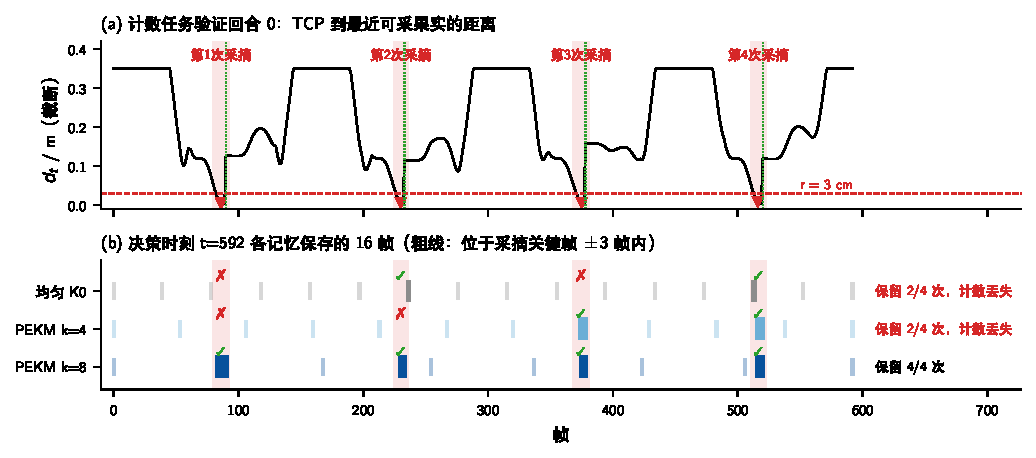
\includegraphics[width=\linewidth]{zh_timeline}
\caption{16 帧记忆实际保存了什么（真实数据，v1 计数任务验证回合 0）。(a) TCP 到最近可采果实的距离 $d_t$，阴影为采摘及其 $\pm 3$ 帧关键窗口，三角为接触关键帧，红色虚线为半径 $r$，绿色点线为果实脱离时刻。(b) 最后一次决策时各记忆保存的帧，粗线表示位于接触或脱离关键帧 $\pm3$ 帧以内，\checkmark/$\times$ 表示该次采摘是否被覆盖。}
\label{fig:timeline}
\end{figure}

\section{HarvestMem 方法}
\label{sec:method}

\subsection{总体框架与设计原则}
\label{sec:framework}
HarvestMem 的总体框架如图~\ref{fig:overview} 所示。它保留通用 VLA 的“视觉编码器 + VLM 骨干 + 记忆分支 + 动作专家”结构，在“\emph{记什么、怎么组织、事件从哪里来}”三个环节引入新设计：\pedet{}（创新一，第~\ref{sec:pedet} 节）回答\emph{何时发生了采摘}；\hem{}（创新二，第~\ref{sec:hem} 节）回答\emph{在固定预算下记住什么、如何编码}；事件鲁棒训练与事后确认自训练（创新三，第~\ref{sec:robust} 节）回答\emph{如何容忍检测误差、如何零标注落地真机}。设计遵循三条原则：

\textbf{P1：事件由物理定义，检测由学习完成。}“什么是一次采摘”由可测量的物理量定义（双指接触、果柄脱离），它在仿真中提供零成本的精确标签，在真机上可由作业结果事后确认；“如何从传感器流中识别它”交给学习型检测器。

\textbf{P2：按事件组织记忆，按时龄分层压缩。}近期事件保留完整细节以支持当下决策，远期事件只保留“在哪里摘过一颗”的摘要证据，场景锚与时间上下文各自占有固定位置。

\textbf{P3：不增加推理开销，可退化为基线。}记忆图像数、token 数和网络主体保持不变；新增嵌入零初始化，训练初始时与基础模型完全等价；当不发生事件时 \hem{} 自动退化为均匀记忆。

\subsection{数据链路与数据流}
\label{sec:dataflow}
图~\ref{fig:dataflow} 给出 HarvestMem 从数据生成到在线控制的完整链路，表~\ref{tab:dataflow} 列出其中流动的主要张量。

\begin{figure}[t]
\centering
\resizebox{\linewidth}{!}{%
\begin{tikzpicture}[font=\footnotesize, >=Stealth,
  nd/.style={draw=black!55, rounded corners=2pt, align=center, text width=2.3cm, minimum height=1.0cm, fill=black!4, font=\footnotesize},
  o1/.style={nd, draw=orange!80!black, thick, fill=orange!12},
  o2/.style={nd, draw=blue!70!black, thick, fill=blue!9},
  o3/.style={nd, draw=green!50!black, thick, fill=green!8},
  lab/.style={fill=white, inner sep=1pt, font=\scriptsize}]
\node[rotate=90, font=\footnotesize\bfseries] at (-0.45,3.55) {训练（离线）};
\node[rotate=90, font=\footnotesize\bfseries] at (-0.45,0.6) {部署（在线，20 Hz）};
\draw[black!25] (-0.2,2.4) -- (15.9,2.4);

\node[nd] (t1) at (1.3,3.2) {程序化场景生成\\{\scriptsize 果树·成熟度·遮挡·风}};
\node[nd] (t2) at (3.95,3.2) {专家示范采集\\{\scriptsize 干净 + DART-H 扰动}};
\node[o1] (t3) at (6.6,3.2) {物理自动标注\\{\scriptsize 接触·脱离·成败，零人工}};
\node[o3] (t4) at (9.25,3.2) {\Ciii{} 事件扰动 EPT\\{\scriptsize 漏检·误检·时间抖动}};
\node[o2] (t5) at (11.9,3.2) {\Cii{} HEM 构造记忆\\{\scriptsize $\{(m_i,\tau_i,\delta_i)\}_{i=1}^{16}$}};
\node[nd] (t6) at (14.55,3.2) {VLA 微调\\{\scriptsize 流匹配损失}};
\node[o1] (tp) at (9.25,4.55) {\Ci{} PEDet 训练\\{\scriptsize + 闭环回放·域随机化}};
\draw[->] (t1) -- (t2); \draw[->] (t2) -- (t3); \draw[->] (t3) -- (t4);
\draw[->] (t4) -- (t5); \draw[->] (t5) -- (t6);
\draw[->] (t3.north) |- (tp.west);

\node[nd] (d1) at (1.3,0.6) {传感器\\{\scriptsize $I^{f}_t,\ I^{w}_t,\ s_t$}};
\node[o1] (d2) at (3.95,0.6) {\Ci{} PEDet 逐帧推理\\{\scriptsize $p^{\mathrm c}_t,\ p^{\mathrm d}_t$}};
\node[o1] (d3) at (6.6,0.6) {迟滞解码\\{\scriptsize 事件表 $\mathcal E_t$}};
\node[o2] (d4) at (9.25,0.6) {\Cii{} HEM（每 16 步）\\{\scriptsize 分层选帧 + 拼图}};
\node[o2] (d5) at (11.9,0.6) {共享视觉编码\\{\scriptsize + 类型-时间嵌入}};
\node[nd] (d6) at (14.55,0.6) {VLA 推理\\{\scriptsize $A_t\in\mathbb R^{20\times8}$ $\rightarrow$ 安全包络 $\rightarrow$ 机械臂}};
\draw[->] (d1) -- (d2); \draw[->] (d2) -- (d3); \draw[->] (d3) -- (d4);
\draw[->] (d4) -- (d5); \draw[->] (d5) -- (d6);
\draw[->] (d1.south) -- ++(0,-0.4) -| node[lab, pos=0.25, below]{帧缓存：每帧 $4{\times}4$ 池化特征（基础结构已有）} ([xshift=-0.5cm]d4.south);
\draw[->, dashed, green!45!black, thick] ([xshift=-0.6cm]d6.north) -- ++(0,0.5) -| node[lab, pos=0.25, above=1pt]{\Ciii{} 事后确认自训练：作业结果 $\rightarrow$ 伪标签 $\rightarrow$ 更新 PEDet（无人工、无附加传感器）} (d2.north);
\draw[->, dashed, black!50] ([xshift=0.6cm]t6.south) -- node[lab, right]{权重} ([xshift=0.6cm]d6.north);
\end{tikzpicture}}
\caption{HarvestMem 的数据链路。上：离线训练链，仿真场景经专家示范、物理自动标注后分两路，一路训练 \pedet，另一路经事件扰动和 \hem{} 构造记忆，形成 VLA 训练样本 $(o_t,s_t,\ell,\mathcal M_t,A^\star_{t:t+20})$。下：在线控制流，\pedet{} 逐帧更新事件表，\hem{} 每次决策时从帧缓存中组织 16 幅记忆图像；回合结束后，作业结果用于事后确认伪标签。训练与部署使用同一个 \hem{} 构造函数。}
\label{fig:dataflow}
\end{figure}

\textbf{离线训练链。}(1) \emph{场景生成}：由布局种子程序化生成果树几何、果实位置与成熟度、遮挡叶片和风的时间表（第~\ref{sec:benchmark} 节）。(2) \emph{示范采集}：规范化专家与相位门控扰动专家（第~\ref{sec:platform} 节）在训练布局上采集示范，每帧记录前置与腕部图像、本体状态、动作标签，以及只用于标注的物理量（指尖接触对、果柄约束标志、果实位姿）。(3) \emph{物理自动标注}：按第~\ref{sec:event_def} 节的定义逐帧生成接触、脱离和成败标签，得到真值事件表 $\mathcal E^\star$。(4) \emph{检测器训练}：用示范和闭环回放训练 \pedet。(5) \emph{记忆构造}：对每个采样到的决策时刻 $t$，先以检测器的误差模型扰动 $\mathcal E^\star$，再由 \hem{} 构造 16 幅记忆图像及其类型和时龄，与当前观测和未来 20 步的专家动作组成训练样本。之所以不直接用 \pedet{} 在训练集上的输出，是因为检测器在自己的训练数据上几乎没有误差，无法反映部署时的真实误差分布（第~\ref{sec:ept} 节）。

\textbf{在线控制流。}每个控制步（20~Hz），前置与腕部图像、本体状态进入帧缓存，帧缓存按基础结构的做法保存每帧经视觉编码器池化后的 16 个 token；\pedet{} 同时对腕部图像和本体状态做一次推理并更新事件表。每 16 步进行一次决策：\hem{} 依据事件表从帧缓存中取出各层记忆帧的特征，摘要层的拼图帧仅在有事件进入摘要层时重新编码一次并缓存；记忆 token 叠加类型-时间嵌入后送入记忆分支，当前两路图像、指令和状态送入骨干，动作专家经 \V{fm_steps} 步流匹配积分输出 $20\times8$ 的动作块，执行前 16 步。回合结束后，事后确认模块根据夹爪与腕部相机记录的作业结果生成伪标签，周期性地更新 \pedet。

\begin{table}[t]
\centering
\caption{HarvestMem 数据流中的主要张量}
\label{tab:dataflow}
\small
\setlength{\tabcolsep}{4pt}
\begin{tabular}{llll}
\toprule
数据 & 形状 & 频率 & 去向\\
\midrule
前置/腕部图像 $I^{f}_t,I^{w}_t$ & $2\times256\times256\times3\rightarrow224\times224$ & 20~Hz & 视觉编码器，每路 256 token\\
腕部图像（检测用） & $128\times128\times3$ & 20~Hz & \pedet{} 视觉分支\\
本体状态 $s_t$ & 8（7 关节角 + 夹爪开度） & 20~Hz & 骨干（离散化 token）、\pedet\\
语言指令 $\ell$ & $\le 200$ token（与状态合计） & 每回合 & 骨干\\
事件概率 $p^{\mathrm c}_t,\,p^{\mathrm d}_t$ & 2 & 20~Hz & 迟滞解码\\
事件表 $\mathcal E_t$ & $\{(t^{\mathrm c}_e,t^{\mathrm d}_e)\}$ & 事件触发 & \hem\\
记忆图像 $\{m_i\}$ & $16\times224\times224\times3$（含拼图帧） & 每 16 步 & 共享视觉编码器\\
记忆 token & $16\times16\times2048$（$4\times4$ 池化） & 每 16 步 & 叠加类型-时间嵌入后进入记忆分支\\
动作块 $A_t$ & $20\times8$（7 关节增量 + 夹爪） & 每 16 步 & 安全包络 $\rightarrow$ 机械臂\\
\bottomrule
\end{tabular}
\end{table}

\subsection{基础策略结构}
\label{sec:base}
策略网络采用当前主流的“视觉-语言骨干 + 动作专家”结构\cite{black2024pi0,pi05_2025}，各部分均不作为本文贡献。当前的前置与腕部图像由冻结的 SigLIP 编码器\cite{zhai2023siglip}编码为每路 256 个 token，与指令和离散化的本体状态一起输入 Gemma-2B 视觉-语言骨干\cite{beyer2024paligemma}。历史记忆由一个约 150M 参数的记忆分支处理：每幅记忆图像经同一 SigLIP 编码后，把 $16\times16$ 的图像块特征平均池化为 $4\times4=16$ 个 token，叠加帧位置编码和该帧的本体状态嵌入；16 幅记忆图像共 256 个 token。约 300M 参数的动作专家以骨干和记忆分支的表示为条件，用流匹配\cite{lipman2023flow}生成 20 步动作块。模型从在通用操作数据上训练的检查点初始化，在 \bench{} 上微调全部非视觉参数。

\subsection{采摘事件的物理定义}
\label{sec:event_def}
一次\emph{采摘事件} $e=(t^{\mathrm c}_e,\,t^{\mathrm d}_e)$ 由两个物理时刻定义：
\begin{itemize}
\item \textbf{接触} $t^{\mathrm c}_e$：夹爪闭合过程中两指首次同时与同一颗果实接触，并持续至少 2 个控制步；
\item \textbf{脱离} $t^{\mathrm d}_e$：该果实的果柄约束解除、且果实仍被夹持的第一个控制步。
\end{itemize}
只有接触之后在时间窗 $T_{\max}$ 内发生脱离，才构成一次\emph{成功采摘}；接触后未脱离（抓空、滑脱、拉拽失败）记为\emph{失败尝试}。该定义不涉及成熟度：摘下青果同样是一次采摘事件，是否该摘是策略的决策问题，而不是记忆组织的问题，这避免了把成熟度真值通过记忆间接泄露给策略。仿真中两个时刻都可从物理状态直接读出，因此标签自动、精确且零成本。作为对照，文献中常用的\emph{几何事件}以 TCP 到最近仍挂树果实的距离
\begin{equation}
d_t=\min_{j\in\mathcal P_t}\lVert p^{\mathrm{TCP}}_t-c_j\rVert_2
\label{eq:signal}
\end{equation}
定义：$d_t\le r$ 的最长连续段构成一个事件（$r=\V{radius_r}$~cm，$\mathrm{tol}=\V{tol}$~mm）。几何事件需要果实位置真值，而且会把每一次失败尝试都记为一次“采摘”。

\subsection{创新一：物理监督的学习型采摘事件检测器 \pedet}
\label{sec:pedet}
\pedet{} 要在不使用任何特权信息的条件下，从机器人自身的传感器流中因果地给出\emph{成功}采摘事件。其结构如图~\ref{fig:pedet} 所示。

\begin{figure}[t]
\centering
\resizebox{\linewidth}{!}{%
\begin{tikzpicture}[font=\footnotesize,
  blk/.style={draw, rounded corners=2pt, align=center, minimum height=0.8cm, inner sep=3pt, fill=white},
  arr/.style={-{Stealth[length=1.8mm]}, thick}]
\node[blk, fill=gray!8] (img) {腕部 RGB\\$128\times128$};
\node[blk, fill=gray!8, below=0.55cm of img] (prop) {本体特征\\$q_t$, $w_t$, $u_t$, $\Delta w_t$};
\node[blk, right=0.5cm of img, fill=blue!6] (cnn) {ResNet-18\\（ImageNet 初始化）};
\node[blk, right=0.5cm of prop, fill=blue!6, minimum width=2.15cm] (mlp) {MLP\\$2\times 64$};
\node[blk, right=0.5cm of cnn, yshift=-0.68cm, fill=blue!6] (fuse) {拼接\\$128+64$};
\node[blk, right=0.5cm of fuse, fill=orange!12, minimum width=2.2cm] (tcn) {因果时序卷积\\4 层，膨胀 1/2/4/8\\感受野 31 帧};
\node[blk, right=0.6cm of tcn, yshift=0.9cm, fill=red!6] (hc) {接触头 $p^{\mathrm c}_t$};
\node[blk, right=0.6cm of tcn, fill=red!6] (hd) {脱离头 $p^{\mathrm d}_t$};
\node[blk, right=0.6cm of tcn, yshift=-0.9cm, fill=gray!6] (hr) {距离头 $\hat d_t$（辅助）};
\node[blk, right=0.5cm of hd, fill=green!6] (dec) {迟滞解码\\成功采摘 $e$\\$(t^{\mathrm c},t^{\mathrm d})$};
\draw[arr] (img) -- (cnn); \draw[arr] (prop) -- (mlp);
\draw[arr] (cnn.east) -- ++(0.2,0) |- (fuse.west);
\draw[arr] (mlp.east) -- ++(0.2,0) |- (fuse.west);
\draw[arr] (fuse) -- (tcn);
\draw[arr] (tcn.east) -- ++(0.25,0) |- (hc.west);
\draw[arr] (tcn) -- (hd);
\draw[arr] (tcn.east) -- ++(0.25,0) |- (hr.west);
\draw[arr] (hc.east) -- ++(0.15,0) |- ([yshift=0.15cm]dec.west);
\draw[arr] (hd) -- (dec);
\node[below=0.25cm of mlp, align=center, text=green!40!black, xshift=1.9cm] {监督信号——仿真：物理状态自动生成；真机：作业结果事后确认（第~\ref{sec:hsl} 节）。两者均无需人工标注};
\end{tikzpicture}}
\caption{\pedet{} 结构。$q_t$ 为关节角，$w_t$ 为夹爪开度，$u_t$ 为夹爪指令，$\Delta w_t$ 为开度变化率。时序卷积只使用当前及过去的帧，检测是因果的。}
\label{fig:pedet}
\end{figure}

\textbf{多模态因果结构。}选择腕部相机，是因为接触和脱离在腕部视角中最清晰，且不受前方叶片遮挡；本体感知则提供与光照无关的“夹住了东西”的证据，两者互补。图像经 ResNet-18\cite{he2016resnet}编码并投影到 128 维，本体特征经两层 MLP 编码为 64 维，拼接后送入 4 层因果时序卷积网络\cite{bai2018tcn,lea2017tcn}（膨胀系数 1、2、4、8，感受野 31 帧，约 1.5~s）。网络有三个输出头：接触概率 $p^{\mathrm c}_t$、脱离概率 $p^{\mathrm d}_t$ 以及截断到 15~cm 的距离估计 $\hat d_t$；距离头只作为辅助任务帮助网络学习“靠近”的几何结构，不参与解码。

\textbf{物理监督与困难负样本。}由第~\ref{sec:event_def} 节的定义，$y^{\mathrm c}_t=1$ 当且仅当两指正与同一果实接触；脱离标签在 $t^{\mathrm d}_e$ 处取 1 并以 $\sigma=1$ 帧的高斯核平滑，以容忍一帧的时间误差；失败尝试的所有帧脱离标签均为 0。训练数据除专家示范外，还加入基础策略在训练布局上的闭环回放，其中大量的抓空、滑脱和重试构成了区分成功与失败所需的\emph{困难负样本}，这是几何定义和手工感知链路都无法提供的。损失函数为
\begin{equation}
\mathcal L_{\mathrm{det}}=\mathcal L_{\mathrm{focal}}(p^{\mathrm c},y^{\mathrm c})+\lambda_{\mathrm d}\,\mathcal L_{\mathrm{focal}}(p^{\mathrm d},\tilde y^{\mathrm d})+\lambda_{\mathrm r}\,\mathbb 1[d_t<0.15]\,\mathrm{SmoothL1}(\hat d_t,d_t),
\end{equation}
其中 focal 损失\cite{lin2017focal}缓解事件帧极度稀少带来的类别不平衡，$\lambda_{\mathrm d}=2$，$\lambda_{\mathrm r}=0.5$。训练时施加域随机化\cite{tobin2017domain}：亮度增益 0.5--1.6、色温偏移、叶片与背景纹理替换、果实色调抖动、腕部相机位姿扰动（$\pm2$~cm、$\pm3^\circ$）、噪声、运动模糊和 JPEG 压缩。

\textbf{因果迟滞解码。}对 $p^{\mathrm c}_t$ 使用迟滞阈值：超过 0.6 进入接触段，低于 0.4 才退出，短于 3 帧的段被丢弃。接触关键帧取接触段开始后 5 帧内 $p^{\mathrm c}_t$ 最大的帧，即夹爪包稳果实的时刻；若接触段内或结束后 5 帧内 $p^{\mathrm d}_t$ 出现超过 0.5 的峰值，以峰值帧为脱离关键帧，确认一次成功采摘；否则记为失败尝试，不进入事件表。进行中的接触段只提供暂定接触帧，保证因果性。

\subsection{创新二：事件中心分层记忆 \hem}
\label{sec:hem}
第~\ref{sec:coverage} 节表明，均匀记忆记得住的采摘次数是一个与作业量无关的常数，而平坦事件关键帧的容量受“每次采摘占两帧”所限。\hem{} 的核心思想是：\textbf{近期事件保细节，远期事件保证据，场景与时间各有其位}。它把 $B$ 个记忆位置组织为四层（图~\ref{fig:hem}）：
\begin{equation}
B=|\mathcal A_t|+|\mathcal W_t|+|\mathcal S_t|+|\mathcal U_t|.
\end{equation}

\begin{figure}[t]
\centering
\resizebox{\linewidth}{!}{%
\begin{tikzpicture}[font=\scriptsize, >=Stealth,
  slot/.style={draw=black!60, minimum width=0.85cm, minimum height=0.85cm, inner sep=0pt},
  sA/.style={slot, fill=teal!25}, sW/.style={slot, fill=orange!35}, sS/.style={slot, fill=blue!18}, sU/.style={slot, fill=black!7}]
\draw[->, thick, black!60] (0,2.6) -- (14.9,2.6) node[right]{$t$};
\node[diamond, draw=teal!70!black, fill=teal!25, inner sep=1.4pt] at (0.25,2.6) {};
\node[above] at (0.25,2.72) {锚};
\foreach \i in {1,...,10} {
  \pgfmathsetmacro{\x}{1.2+(\i-1)*1.38}
  \ifnum\i<9
    \node[circle, draw=blue!70!black, fill=blue!18, inner sep=1.6pt] at (\x,2.6) {};
  \else
    \node[circle, draw=orange!80!black, fill=orange!35, inner sep=1.6pt] at (\x,2.6) {};
  \fi
  \node[above] at (\x,2.72) {$e_{\i}$};
}
\draw[decorate, decoration={brace, mirror, amplitude=4pt}] (1.0,2.4) -- (5.55,2.4) node[midway, below=4pt] (b1) {拼图帧 $S_1$};
\draw[decorate, decoration={brace, mirror, amplitude=4pt}] (6.5,2.4) -- (11.07,2.4) node[midway, below=4pt] (b2) {拼图帧 $S_2$};
\draw[decorate, decoration={brace, mirror, amplitude=4pt}] (12.0,2.4) -- (13.8,2.4) node[midway, below=4pt] (b3) {工作层 $\mathcal W$};

\foreach \j/\sty/\txt in {0/sA/{$I_0$}, 1/sS/{}, 2/sS/{}, 3/sW/{$c_9$}, 4/sW/{$d_9$}, 5/sW/{$c_{10}$}, 6/sW/{$d_{10}$}} {
  \node[\sty] (s\j) at (\j*0.93+0.425,0.6) {\txt};
}
\foreach \j in {7,...,15} { \node[sU] (s\j) at (\j*0.93+0.425,0.6) {$u$}; }
\foreach \j/\a/\b/\c/\d in {1/1/2/3/4, 2/5/6/7/8} {
  \draw[black!50] (s\j.north) -- (s\j.south); \draw[black!50] (s\j.west) -- (s\j.east);
  \node[font=\tiny] at ([xshift=-0.21cm, yshift=0.21cm]s\j.center) {\a};
  \node[font=\tiny] at ([xshift=0.21cm, yshift=0.21cm]s\j.center) {\b};
  \node[font=\tiny] at ([xshift=-0.21cm, yshift=-0.21cm]s\j.center) {\c};
  \node[font=\tiny] at ([xshift=0.21cm, yshift=-0.21cm]s\j.center) {\d};
}
\draw[->, black!50] (b1.south) -- (s1.north);
\draw[->, black!50] (b2.south) -- (s2.north);
\draw[->, black!50] (b3.south) -- ([xshift=0.45cm]s4.north);
\draw[->, black!50] (0.25,2.45) -- (s0.north);
\draw[decorate, decoration={brace, mirror, amplitude=4pt}] ([yshift=-0.08cm]s7.south west) -- ([yshift=-0.08cm]s15.south east) node[midway, below=4pt] {时间上下文层 $\mathcal U$：其余帧中等距选取（含失败尝试、场景演变）};
\node[anchor=north west, align=left] at (-0.05,-0.7) {\sq{teal!70!black} 场景锚 $\mathcal A$\quad \sq{blue!70!black} 情景摘要 $\mathcal S$（每格 $112^2$，对齐 $2\times2$ token）\\ \sq{orange!80!black} 工作事件 $\mathcal W$（接触 $c$ / 脱离 $d$）\quad \sq{black!40} 时间上下文 $\mathcal U$};
\end{tikzpicture}}
\caption{\hem{} 的记忆布局示例（第 10 次采摘之后的决策时刻，$B=16$）。最近 2 次采摘保留完整的接触帧与脱离帧；更早的 8 次采摘被压缩进 2 幅事件拼图帧，每格是一次采摘脱离后以 TCP 为中心的局部图像；第 0 帧作为场景锚；其余 9 个位置按时间等距选取。同样的 16 个位置，均匀记忆平均只能覆盖约 \V{cap_u} 次采摘，平坦关键帧（$k=8$）只能覆盖 4 次。}
\label{fig:hem}
\end{figure}

\textbf{场景锚层 $\mathcal A_t$。}包含第 0 帧以及最近一次场景切换（如换到下一株植物）后的第一帧，最多 2 个位置。场景切换时刻由平台的移动信号给出，不需要视觉检测。这一层承载场景记忆：叶片被风吹动之前看到的成熟果实。

\textbf{工作事件层 $\mathcal W_t$。}最近 $m_w=\V{hem_mw}$ 次成功采摘的接触帧与脱离帧，以完整分辨率保留“刚刚做了什么”的细节，支持避免重复抓取同一颗果、确认刚才的放果等即时决策。

\textbf{情景摘要层 $\mathcal S_t$ 与事件拼图帧。}更早的采摘按时间分组，每 $c=\V{hem_c}$ 次合成一幅\emph{事件拼图帧}，最多 $s_{\max}=\V{hem_smax}$ 幅。对事件 $e$，取其脱离后第 3 帧的前置图像，以 TCP 的图像投影为中心裁出局部区域并缩放到 $112\times112$，作为“在这里摘下过一颗果”的证据；4 个局部图像按时间顺序拼为一幅 $224\times224$ 图像，空格以中性灰填充并在注意力中屏蔽。拼图帧有一个关键的结构性质：SigLIP 把 $224\times224$ 图像切成 $16\times16$ 个图像块，记忆分支再平均池化为 $4\times4$ 个 token，因此每个 $112\times112$ 格恰好对应 $8\times8$ 个图像块、池化后的 $2\times2$ 个 token，\textbf{格与格之间在池化时互不混叠}。于是拼图帧在不增加 token、不引入新编码器的前提下，把 4 次采摘的证据装进一个记忆位置。远期事件只需回答“是否摘过、在哪里摘过”，不需要操作细节，较低的分辨率足以满足需要。

\textbf{时间上下文层 $\mathcal U_t$。}其余位置在不属于前三层的帧中等距选取，保留场景演变、失败尝试和回合进度的连续信息。

\textbf{自适应预算分配。}各层的位置数随事件数 $n$ 自动调整：
\begin{equation}
|\mathcal W_t|=2\min(n,m_w),\qquad |\mathcal S_t|=\Big\lceil \frac{\min\big(\max(n-m_w,0),\ c\,s_{\max}\big)}{c}\Big\rceil,\qquad |\mathcal U_t|=B-|\mathcal A_t|-|\mathcal W_t|-|\mathcal S_t|.
\end{equation}
回合初期尚无事件时，几乎全部位置用于时间上下文，\hem{} 退化为均匀记忆；事件累积后，事件层至多占用 $2m_w+s_{\max}=7$ 个位置，时间上下文始终保留至少 7 个位置。构造过程见算法~\ref{alg:hem}。

\begin{algorithm}[t]
\caption{\hem{} 在决策时刻 $t$ 的记忆构造}
\label{alg:hem}
\small
\begin{algorithmic}[1]
\Require 帧缓存 $I_{0:t}$，成功采摘事件表 $\mathcal E_t=(e_1,\dots,e_n)$，场景切换时刻 $t^{\mathrm s}$，预算 $B$，参数 $m_w,c,s_{\max}$
\Ensure 记忆 $\mathcal M_t=\{(m_i,\tau_i,\delta_i)\}_{i=1}^{B}$
\If{$t+1\le B$} \Return $\{(I_f,\textsc{上下文},t-f)\}_{f=0}^{t}$ \EndIf
\State $\mathcal A\gets\{0,\ t^{\mathrm s}\}$ \Comment{场景锚}
\State $\mathcal W\gets\{(t^{\mathrm c}_e,\textsc{接触}),\ (t^{\mathrm d}_e,\textsc{脱离}):\ e\in(e_{n-m_w+1},\dots,e_n)\}$ \Comment{工作事件层}
\State $\mathcal O\gets(e_{\max(1,\,n-m_w-c\,s_{\max}+1)},\dots,e_{n-m_w})$ \Comment{进入摘要层的事件}
\For{$\mathcal O$ 中按时间顺序每 $c$ 个事件组成的组 $g$}
  \State $m_g\gets\textsc{Mosaic}\big(\{\textsc{Crop}(I^{f}_{t^{\mathrm d}_e+3},\ \mathrm{TCP}_{t^{\mathrm d}_e+3}):e\in g\}\big)$，加入 $\mathcal S$ \Comment{事件拼图帧}
\EndFor
\State $n_U\gets B-|\mathcal A|-|\mathcal W|-|\mathcal S|$；$R\gets\{0,\dots,t\}\setminus(\mathcal A\cup\mathcal W)$
\State $\mathcal U\gets\{R[\lfloor i(|R|-1)/(n_U-1)\rfloor]:\ i=0,\dots,n_U-1\}$ \Comment{时间上下文层}
\State \Return $\mathcal A\cup\mathcal W\cup\mathcal S\cup\mathcal U$ 按时间排序，附类型 $\tau$ 与时龄 $\delta=t-f$
\end{algorithmic}
\end{algorithm}

\textbf{类型-时间嵌入。}分层之后，同一个记忆位置上可能是场景锚、接触瞬间、脱离瞬间、拼图帧或普通上下文帧，策略需要知道每幅记忆“是什么、多久以前”。基础结构中的帧位置编码只表示排列顺序，无法表达这些信息。为此，对记忆图像 $i$ 的第 $j$ 个 token，在视觉特征 $h_{i,j}$ 上叠加
\begin{equation}
z_{i,j}=h_{i,j}+\mathbf e_{\tau_{i,j}}+g\big(\phi(\delta_{i,j})\big),\qquad \tau\in\{\text{锚},\text{接触},\text{脱离},\text{摘要},\text{上下文}\},
\end{equation}
其中 $\mathbf e_\tau\in\mathbb R^{2048}$ 为可学习的类型嵌入，$\phi(\delta)$ 是 $\log(1+\delta)$ 的 16 频正弦特征，$g$ 为 $32\rightarrow64\rightarrow2048$ 的两层 MLP。对拼图帧，每个格对应的 $2\times2$ 个 token 各自使用该格事件的时龄，因此一幅拼图帧内的 4 次采摘仍可区分先后。类型嵌入和 $g$ 的最后一层均\emph{零初始化}，训练开始时模型与基础模型完全等价，新增参数仅约 \V{hem_params}~M。

\textbf{性质。}\hem{} 具有以下性质。\emph{预算与开销不变}：恒输出 $B$ 幅记忆图像、$16B$ 个 token；拼图帧只在有事件进入摘要层时编码一次，构造耗时约 \V{hem_ms}~ms。\emph{严格包含基线}：$m_w=s_{\max}=0$ 时即均匀记忆，$s_{\max}=0$ 时即平坦事件关键帧。\emph{因果且训练部署一致}：只使用已确认的事件，训练样本与在线决策调用同一构造函数。其事件容量由下述命题给出。

\begin{proposition}[分层记忆的事件容量]
\label{prop:capacity}
若事件检测正确，则在任意决策时刻，\hem{} 保留最近 $\min(n,\ m_w+c\,s_{\max})$ 次采摘的直接证据，至多占用 $2m_w+s_{\max}$ 个事件位置；占用同样多位置的平坦事件关键帧至多保留 $\lfloor(2m_w+s_{\max})/2\rfloor$ 次。
\end{proposition}
\noindent 取 $B=16$、$m_w=2$、$c=4$、$s_{\max}=3$，\hem{} 用 7 个事件位置保留 \V{cap_hem} 次采摘，平坦方案用 8 个位置只保留 4 次，且容量可通过 $c$ 和 $s_{\max}$ 继续扩展。图~\ref{fig:capacity} 在合成事件序列上验证了这一点：均匀记忆平均只覆盖约 \V{cap_u} 次采摘，平坦关键帧在第 4 次之后饱和于约 \V{cap_k8} 次，\hem{} 在 14 次以内全部覆盖。

\begin{figure}[t]
\centering
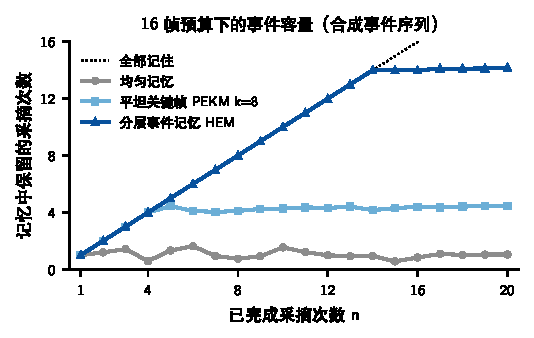
\includegraphics[width=0.62\linewidth]{zh_capacity}
\caption{16 帧记忆预算下保留的采摘次数（真实计算）。合成事件序列中相邻采摘间隔服从 $U(110,190)$ 帧，每个 $n$ 重复 300 次；某次采摘被计为保留，当且仅当记忆中有一帧落在其接触或脱离帧 $\pm3$ 帧内，或该采摘位于拼图帧中。}
\label{fig:capacity}
\end{figure}

\subsection{创新三：事件鲁棒训练与免标注真机适配}
\label{sec:robust}

\subsubsection{事件扰动训练（EPT）}
\label{sec:ept}
训练时若直接使用物理真值事件，策略看到的记忆永远“完美”，会学会无条件信任记忆；而部署时 \pedet{} 不可避免地存在少量漏检、误检和时间偏差，例如漏掉一次脱离会让记忆中少一次采摘，诱发多摘。我们提出\emph{事件扰动训练}：以概率 $\rho=0.5$ 对每个训练样本的真值事件表 $\mathcal E^\star$ 施加扰动 $\tilde{\mathcal E}=\Pi(\mathcal E^\star)$，包括 (1) 以概率 $p_{\mathrm{miss}}$ 删除事件；(2) 以概率 $p_{\mathrm{fp}}$ 把失败尝试误标为成功采摘，若该回合无失败尝试，则在接近阶段随机插入；(3) 把每个关键帧在 $\{-2,\dots,2\}$ 帧内随机偏移。扰动率按检测器在真机上的误差水平设定（$p_{\mathrm{miss}}=p_{\mathrm{fp}}=0.05$），比仿真误差更保守。被删除的事件仍可能出现在时间上下文层中，于是策略学会把事件层与上下文层、当前观测相互印证，而不是盲信任何单一来源。

\subsubsection{事后确认自训练（HSL）}
\label{sec:hsl}
真机上没有仿真物理状态，人工逐帧标注接触与脱离又费时费力；在果实或植株上加装传感器在生产中也不可行。我们的关键观察是：\textbf{一次采摘是否成功，在发生的瞬间难以判断，但在事后很容易确认}——成功的采摘必然以“夹着果实到达集果篮并松开”结束。据此提出\emph{事后确认自训练}，只使用夹爪开度、腕部相机和标定一次的篮区位置：
\begin{enumerate}
\item \textbf{持物段提取。}夹爪闭合指令发出后，若开度在 5 帧以上停滞在果实尺寸对应的区间内，即判定夹爪中有物体，记为一个持物段 $[t_a,t_b]$。
\item \textbf{结果确认。}若段末夹爪在篮区上方张开，且腕部图像中两指之间区域由“有果”变为“空”（与张开前相比的像素差超过阈值），确认为\emph{成功}；若开度在到达篮区之前塌缩到全闭（滑脱），或在篮区外张开，确认为\emph{失败}；闭合后开度直接到底的抓空同样记为失败。
\item \textbf{时刻回溯。}成功段的接触帧取持物段起点，脱离帧取段内当前 \pedet{} 的 $p^{\mathrm d}_t$ 最大值；若机械臂提供关节电流，拉拽时的电流峰值可作为辅助证据。失败段内所有帧的脱离标签为 0，构成纠正误检的困难负样本。
\item \textbf{一致性筛选与迭代。}只保留脱离帧位于拉拽阶段（TCP 离开接触位置 5~cm 之前）且 $\max p^{\mathrm d}_t>0.3$ 的成功段；用伪标签与仿真数据混合微调 \pedet{}（冻结视觉骨干前三个阶段），再用更新后的检测器重新回溯脱离帧，共迭代 2 轮。
\end{enumerate}
HSL 不需要任何人工标注，也不需要在果实、果柄或植株上加装传感器，可以在日常作业中持续运行，使检测器随作物、季节和光照的变化自我更新。在真机实验中，\pct{hsl_keep} 的持物段通过一致性筛选，伪标签相对人工标注的事件精确率为 \V{hsl_prec}（第~\ref{sec:res_real} 节）。

\subsection{低层执行平台}
\label{sec:platform}
\label{sec:dart}
记忆方法能否在闭环中体现价值，取决于低层执行是否可靠。早期实验中，策略常在搬运和放果后出现腕关节大幅偏转、长时间停滞等问题，成败主要由操作失误决定。为此，我们对执行平台做了四项改进并在训练前冻结：(1) \emph{规范化专家}：基于 mplib\cite{mplib}的脚本专家以固定休息位姿作为逆运动学初值，分区设置碰撞裕度并加入收臂路点，消除示范中的多峰腕部姿态；(2) \emph{相位门控恢复示范（DART-H）}：参照 DART\cite{laskey2017dart}，只在接近、搬运等自由运动阶段注入 Ornstein--Uhlenbeck 关节噪声（$\sigma=0.04$~rad，$\tau=10$ 步），记录从扰动状态重新规划的干净动作作为标签，以缓解协变量偏移\cite{ross2011dagger}；(3) \emph{观察期保持}：回合前 30 步机械臂静止，这些帧只作为历史进入记忆；(4) \emph{安全包络}：把关节目标裁剪到示范分布的 [0.5\%, 99.5\%] 分位区间外扩 0.1~rad，并限制单步增量。在 dev 布局上，这些改进使均匀记忆策略的整任务成功率从 \pct{ll_succ_a} 提高到 \pct{ll_succ_b}，首颗果实入篮率从 \pct{ll_first_a} 提高到 \pct{ll_first_b}，腕部失控率从 \pct{ll_wrist_a} 降到 \pct{ll_wrist_b}，放果后恢复运动的中位步数从 \V{ll_resume_a} 降到 \V{ll_resume_b}。所有记忆条件共用同一平台。

\section{\bench{} 基准及其有效性审计}
\label{sec:benchmark}

\subsection{场景、机器人与传感}
\bench{} 基于 ManiSkill3\cite{tao2025maniskill3}构建。每个回合随机生成一棵带主干、枝条和叶簇的果树，挂有 4--6 颗半径 2.5--2.9~cm 的球形果实，果实高度 0.44--0.64~m，距机器人基座 0.38--0.50~m，方位角在 $\pm28^\circ$ 以内。布局采样器保证每颗果实都存在水平接近的逆运动学解、接近通道内没有枝条，且果实在前置相机中互不遮挡。果实被双指连续夹持 2 个控制步后脱离果柄，成为自由刚体。机器人为睿尔曼 RM75-B 七自由度机械臂加 EG2 两指夹爪，关节位置控制，控制频率 20~Hz。观测包括前置和腕部两台 RGB-D 相机（$256\times256$ 像素，前置视场角 $55^\circ$，腕部 $90^\circ$）以及 8 维本体状态（7 个关节角和 1 个夹爪开度）。集果篮位于机器人侧方，始终在前置相机视野之外。图~\ref{fig:scene} 为真实渲染画面。

\begin{figure}[t]
\centering
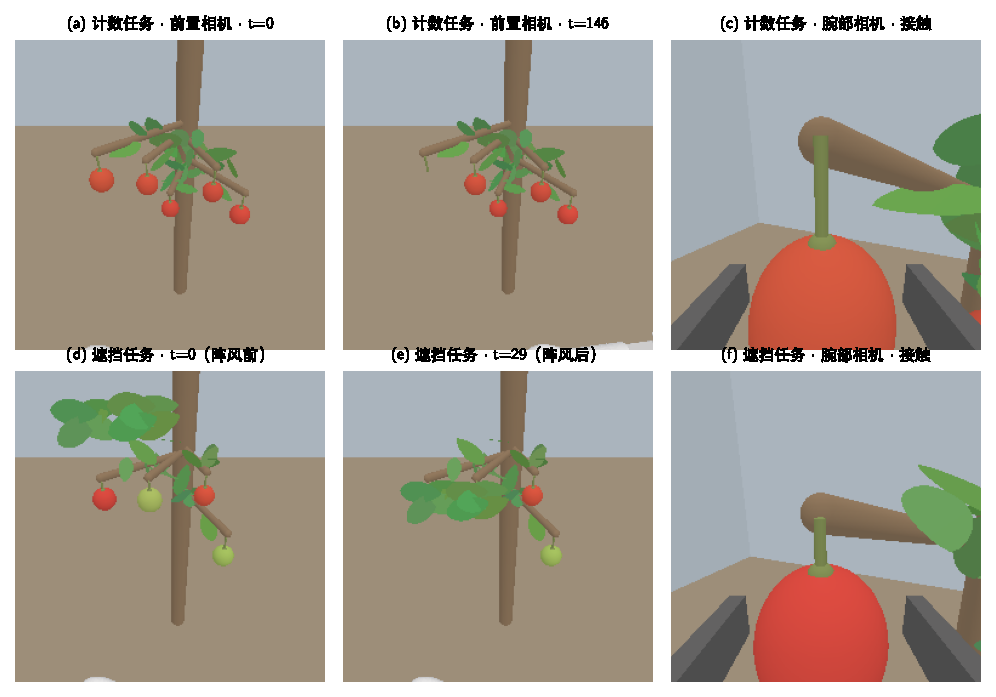
\includegraphics[width=0.86\linewidth]{zh_scene}
\caption{\bench{} 场景（真实渲染，v1 任务）。(a)--(c) 计数任务：开始时与一次采摘后的前置相机画面，以及接触时刻的腕部画面；(d)--(f) 遮挡任务：阵风前后的前置相机画面（阵风后两个叶簇遮住果实）以及接触时刻的腕部画面。v2 任务在此基础上增加风落果和颜色褪变（图~\ref{fig:tasks}）。}
\label{fig:scene}
\end{figure}

\subsection{原始任务为何检测不出记忆差异}
\label{sec:v1}
基准的第一版（v1）包含两个任务。\textbf{计数任务}要求在 $M$ 颗成熟果中恰好摘 $N$ 颗（$N=2$--5），入篮数达到 $N$ 即判成功。\textbf{遮挡任务}中红果与青果混挂，观察阶段第 8--20 步的一阵风把两个叶簇吹到两颗果实前方，指令要求把所有成熟果放入篮中、不放青果。按设计，前者需要记住自己摘了几颗，后者需要记住被遮住的果实是否成熟。

我们按预先登记的协议，在 val 50--99 布局 $\times$ 3 个种子（每格 \V{v1_n} 次）上比较了 K0（均匀记忆）与 K4、K8（平坦事件关键帧 \pekm{}，几何事件）三种策略。结果如表~\ref{tab:v1} 所示：四项主假设均未获支持，Holm 校正后 $p=\V{v1_holm}$。事后诊断找到了三个原因：
\begin{enumerate}
\item \textbf{计数任务在达到配额时自动结束。}仿真环境在成功或失败时立即终止回合，入篮数一旦等于 $N$ 就判成功，策略根本没有“多摘”的机会；这类记忆失败在结构上恒为 \V{v1_cnt_memfail}。
\item \textbf{遮挡任务可以靠当前画面完成。}叶簇本身标出了被遮果实的位置，被遮果实中 \pct{v1_hidden_ripe_frac} 是成熟的；更关键的是，叶片在 TCP 进入 15~cm 范围时会被推开，K0 接近被遮挡成熟果时有 \pct{v1_leaf_lift} 的情况叶片抬起、露出果实颜色。策略只需“走近看一眼”。
\item \textbf{场景信息天然被均匀记忆保留。}均匀采样总是包含第 0 帧，阵风前的画面在三种记忆的所有决策中都被保留（\pct{v1_frame0}），因此三者在场景信息上没有差别；在推理时去掉阵风前的帧，遮挡任务成功率仅从 \pct{v1_nopregust_a} 降到 \pct{v1_nopregust_b}。
\end{enumerate}
结论是：v1 的零结果说明这个基准检测不出记忆差异，而不能说明事件关键帧无效。这一教训促使我们在评估任何记忆方法之前，先审计任务是否真的需要记忆。

\begin{table}[t]
\centering
\caption{v1 原始任务上的预登记正式评测（真实结果；每格 150 次，val 50--99 $\times$ 种子 7/8/9）}
\label{tab:v1}
\small
\begin{tabular}{lcccl}
\toprule
任务 & K0 均匀 & K4 & K8 & 诊断\\
\midrule
计数（v1） & \pct{v1_cnt_k0} & \pct{v1_cnt_k4} & \pct{v1_cnt_k8} & 达到配额即终止，多摘失败结构性为 0\\
遮挡（v1） & \pct{v1_occ_k0} & \pct{v1_occ_k4} & \pct{v1_occ_k8} & 叶片靠近即抬起，颜色可见\\
遮挡错果率 & \pct{v1_occ_wrong_k0} & \pct{v1_occ_wrong_k4} & \pct{v1_occ_wrong_k8} & 第 0 帧在所有决策中均被保留\\
\bottomrule
\end{tabular}
\end{table}

\subsection{v2 任务：把场景记忆与事件记忆分开}
\label{sec:tasks}
v2 的设计目标有三条：无记忆策略的成功率必须很低；场景记忆与事件记忆分开检验，并把预测事先写入协议；事件数量要足够多，能够检验记忆容量（图~\ref{fig:tasks}）。

\textbf{计数 v2（事件记忆）。}取消“入篮数等于 $N$ 即结束”。回合在以下任一情况结束：策略发出\emph{完成信号}（回到休息位姿附近、夹爪张开、未持果，且静止至少 40 步）；达到步数预算；入篮数超过 $N$（立即判失败）；机器人掉果（立即判失败）。成功定义为结束时入篮数恰好为 $N$ 且没有掉果。为堵住“开头数总果数 $M$、当前数剩余果数 $R$、用 $M-R$ 推算已摘数”的捷径，回合中途会随机让 1--2 颗未被摘取的果实被风吹落到地面；风落果单独标记，不算机器人掉果，也不会落入篮中。于是“已摘几颗”只存在于机器人自己每次放果的短暂时刻中，这正是事件记忆的情形。专家在放完第 $N$ 颗后回到休息位姿并保持静止。

\textbf{遮挡 v2（场景记忆）。}阵风期间（第 8--20 步），所有果实的外观颜色逐渐褪变为同一种中性色，两台相机此后都无法再分辨成熟度，成熟度信息只存在于阵风前的画面中；叶簇保留。成功定义不变：所有成熟果入篮，且没有青果入篮。由于均匀记忆总是保留第 0 帧，而 \hem{} 的场景锚层同样保留第 0 帧，我们\emph{预测}该任务上各记忆条件之间没有差异。这一任务用作“不伤害场景记忆”的等效性检验。

\textbf{多株长时配额 FruitRow（长时事件记忆）。}模拟沿种植行连续作业的场景：一行 3 株植物，每株挂 3--5 颗成熟果和若干青果，指令要求整行共摘 $N$ 颗成熟果（$N=6$--12）。当前株已无可摘成熟果时，平台把下一株移到机器人前方（仿真中替换场景并发出换株信号），此前的植株随即离开视野。风落果机制与计数 v2 相同，回合同样由完成信号结束。平均每回合 \V{row_events} 次采摘、\V{row_steps} 个控制步，远超平坦事件关键帧的容量。由于前面植株上的采摘既不可见、也无法从当前株推算，记住整行的累计采摘次数只能依靠长时事件记忆。

\begin{figure}[t]
\centering
\resizebox{\linewidth}{!}{%
\begin{tikzpicture}[font=\footnotesize, x=0.0103cm, y=1cm]
\def\L{1000}
% count v2
\node[anchor=east, align=right] at (-20,0) {\textbf{计数 v2}\\事件记忆};
\draw[thick,-{Stealth}] (0,0) -- (\L,0);
\fill[gray!25] (0,-0.18) rectangle (30*2.2,0.18);
\node[above] at (33,0.18) {观察};
\foreach \x/\n in {190/1,390/2,600/3}{
  \fill[blue!60] (\x,-0.18) rectangle (\x+14,0.18);
  \node[above, text=blue!60!black] at (\x+7,0.18) {放果 \n};
}
\foreach \x in {300,520}{
  \draw[red!70!black, thick] (\x,-0.32) -- (\x,0.32);
  \node[below, text=red!70!black] at (\x,-0.3) {风落果};
}
\fill[green!50!black!50] (760,-0.18) rectangle (900,0.18);
\node[above, text=green!40!black] at (830,0.18) {完成信号（静止 $\ge$40 步）};
\node[anchor=west, align=left, text=gray!40!black] at (1010,0) {篮子不在前置视野；\\$M-R\neq$ 已摘数};
% occluded v2
\node[anchor=east, align=right] at (-20,-1.25) {\textbf{遮挡 v2}\\场景记忆};
\draw[thick,-{Stealth}] (0,-1.25) -- (\L,-1.25);
\shade[left color=red!60, right color=gray!50] (8*2.2,-1.43) rectangle (20*2.2,-1.07);
\fill[gray!25] (0,-1.43) rectangle (8*2.2,-1.07);
\fill[gray!25] (20*2.2,-1.43) rectangle (30*2.2,-1.07);
\node[above] at (33,-1.07) {阵风+褪色};
\foreach \x/\n in {200/1,430/2}{
  \fill[blue!60] (\x,-1.43) rectangle (\x+14,-1.07);
  \node[above, text=blue!60!black] at (\x+7,-1.07) {采摘 \n};
}
\fill[gray!50] (66,-1.55) rectangle (\L,-1.5);
\node[below, text=gray!40!black] at (520,-1.5) {此后所有果实为同一中性色，成熟度只存在于阵风前画面};
\node[anchor=west, align=left, text=gray!40!black] at (1010,-1.25) {均匀记忆与场景锚均保留第 0 帧；\\预测各记忆条件无差异};
% FruitRow
\node[anchor=east, align=right] at (-20,-2.6) {\textbf{FruitRow}\\长时事件记忆};
\draw[thick,-{Stealth}] (0,-2.6) -- (\L,-2.6);
\foreach \a/\b/\n in {0/330/1,345/665/2,680/985/3}{
  \fill[green!12] (\a,-2.78) rectangle (\b,-2.42);
  \node[above, text=green!35!black] at ({(\a+\b)/2},-2.42) {第 \n 株};
}
\foreach \x in {337,672}{ \draw[black!70, very thick, densely dashed] (\x,-2.86) -- (\x,-2.34); }
\node[below, text=black!60] at (504,-2.86) {换株：前面植株离开视野};
\foreach \x in {60,120,190,255,400,470,540,610,730,800}{ \fill[blue!60] (\x,-2.78) rectangle (\x+10,-2.42); }
\draw[red!70!black, thick] (430,-2.92) -- (430,-2.28);
\fill[green!50!black!50] (880,-2.78) rectangle (970,-2.42);
\node[anchor=west, align=left, text=gray!40!black] at (1010,-2.6) {平均 \V{row_events} 次采摘；\\超出平坦关键帧容量};
\draw[-{Stealth}] (0,-3.45) -- (150,-3.45) node[right] {控制步（示意）};
\end{tikzpicture}}
\caption{v2 三个任务的时间结构（示意）。计数 v2 中，回合由策略的完成信号结束，中途的风落果使“开头果数减当前果数”不再等于已摘数；遮挡 v2 中，阵风期间颜色褪变，成熟度只存在于开头画面中；FruitRow 中采摘分布在 3 株植物上，换株后前面植株离开视野，时间轴按比例压缩。}
\label{fig:tasks}
\end{figure}

\subsection{信息受限脚本策略的捷径审计}
\label{sec:audit}
为检验任务是否真的需要相应的记忆，我们构造三种基于真值的脚本策略，它们使用相同的专家运动规划，只是能用于\emph{决策}的信息不同：(O1) 只用当前帧可见的信息；(O2) 第 0 帧加当前帧；(O3) 完整历史，即专家本身。每个任务每种策略各在 \V{audit_n} 个 dev 布局上运行。事先规定的通过标准是：计数 v2 与 FruitRow 中 O1 和 O2 的成功率都不高于 30\%，O3 不低于 90\%（FruitRow 的 O2 使用当前株的第一帧）；遮挡 v2 中 O1 不高于 30\%，O2 和 O3 都不低于 90\%（场景记忆按设计只需第 0 帧）。此外要求专家逐尝试成功率不低于 90\%，示范通过安全包络时的裁剪率低于 0.5\%。

审计结果见表~\ref{tab:audit}，三个任务均达到预设标准。计数 v2 中，只看当前帧的策略无从知道已摘几颗，典型失败是持续采摘直到超额；看第 0 帧的策略会用 $M-R$ 估计已摘数，被风落果误导，典型失败为少摘后提前发出完成信号。遮挡 v2 中，只看当前帧的策略只能在同色果实间猜测成熟度，成功率接近随机猜测水平；只要能看到第 0 帧，成功率就与完整历史相当。FruitRow 上 O1、O2 几乎全部失败，因为前面植株上的采摘无从推算。这说明计数 v2 与 FruitRow 检验的是事件记忆，遮挡 v2 检验的是场景记忆，与设计一致。

事件信号本身也需要审计。v1 中的几何事件只计算到“成熟且仍挂树”的果实的距离，用到了成熟度真值，可能通过选帧间接向策略提示成熟度。v2 中我们统一采用第~\ref{sec:event_def} 节与成熟度无关的物理事件定义，训练与评测的所有记忆条件使用同一定义。

\begin{table}[t]
\centering
\caption{v2 任务的捷径审计（每格 \V{audit_n} 个 dev 布局）}
\label{tab:audit}
\small
\setlength{\tabcolsep}{3pt}
\begin{tabular}{lcccl}
\toprule
任务 & O1 仅当前帧 & O2 首帧+当前帧 & O3 完整历史 & 预设标准\\
\midrule
计数 v2（事件记忆） & \pct{aud_cnt_o1} & \pct{aud_cnt_o2} & \pct{aud_cnt_o3} & O1、O2 $\le$30\%；O3 $\ge$90\%\\
遮挡 v2（场景记忆） & \pct{aud_occ_o1} & \pct{aud_occ_o2} & \pct{aud_occ_o3} & O1 $\le$30\%；O2、O3 $\ge$90\%\\
FruitRow（长时事件记忆） & \pct{aud_row_o1} & \pct{aud_row_o2} & \pct{aud_row_o3} & O1、O2 $\le$30\%；O3 $\ge$90\%\\
\midrule
\multicolumn{5}{l}{专家逐尝试成功率（计数 v2 / 遮挡 v2 / FruitRow）：\pct{exp_cnt} / \pct{exp_occ} / \pct{exp_row}；示范裁剪率：\pct{clip_cnt} / \pct{clip_occ}}\\
\bottomrule
\end{tabular}
\end{table}

\section{实验设计}
\label{sec:design}

\subsection{研究问题}
实验围绕六个问题展开：
\begin{itemize}
\item \textbf{RQ1}：固定预算的记忆实际保留了哪些信息？均匀记忆的事件覆盖率是否符合命题~\ref{prop:uniform}？
\item \textbf{RQ2}：\pedet{} 能否在不使用特权信息的条件下准确检测采摘事件、区分成功与失败尝试，并对光照变化鲁棒？
\item \textbf{RQ3}：\hem{} 能否提高依赖事件记忆的任务成功率，同时不损害依赖场景记忆的任务？
\item \textbf{RQ4}：当采摘次数超出平坦关键帧的容量时，分层记忆是否仍然有效？
\item \textbf{RQ5}：增益是否来自事件内容本身？各组件是否必要？
\item \textbf{RQ6}：上述结论能否迁移到真实番茄采摘？检测器能否不用人工标注完成真机适配？
\end{itemize}

\subsection{对比条件与训练设置}
主实验比较四种记忆条件：\textbf{K0}（均匀记忆，即基础模型）；\textbf{K4}、\textbf{K8}（平坦事件关键帧，预留 4 或 8 帧）；\textbf{HEM}（完整的 HarvestMem）。为使比较只反映记忆组织方式的差异，K4、K8 与 HEM 使用相同的 \pedet{} 事件和相同的事件扰动训练，HEM 额外包含分层结构、拼图帧和类型-时间嵌入。每个 v2 任务生成干净专家示范 100 个（train 0--99）和 DART-H 恢复示范 100 个（train 100--199），dev 200--259 用于调试，正式评测使用从未用过的 val 150--199。四种条件的其余设置完全相同（表~\ref{tab:train}）。

\begin{table}[t]
\centering
\caption{训练设置（各记忆条件相同）}
\label{tab:train}
\small
\setlength{\tabcolsep}{4pt}
\begin{tabular}{ll|ll}
\toprule
\multicolumn{2}{c|}{VLA 策略} & \multicolumn{2}{c}{\pedet}\\
\midrule
初始化 & 通用操作数据检查点 & 视觉骨干 & ResNet-18（ImageNet）\\
训练步数 & \V{train_steps} & 时序模块 & 4 层因果 TCN\\
全局批大小 & 64 & 序列长度 & 64 帧\\
优化器 & AdamW，梯度裁剪 1.0 & 优化器 & AdamW，$3\times10^{-4}$\\
学习率 & 预热 500 步至 $2.5\times10^{-5}$，余弦衰减 & 训练轮数 & 30\\
EMA / 视觉编码器 & 0.999 / 冻结 & 批大小 & 128 段\\
事件扰动 EPT & $\rho=0.5$，$p_{\mathrm{miss}}=p_{\mathrm{fp}}=0.05$，$\pm2$ 帧 & 数据 & 示范 + 闭环回放\\
\hem{} 参数 & $m_w=\V{hem_mw}$，$c=\V{hem_c}$，$s_{\max}=\V{hem_smax}$ & 增广 & 域随机化（第~\ref{sec:pedet} 节）\\
新增参数 & 类型-时间嵌入约 \V{hem_params}~M，零初始化 & 真机适配 & HSL，\V{rb_hsl_ep} 个无标注回合\\
硬件 & 8 $\times$ NVIDIA L20（FSDP） & 硬件 & 1 $\times$ NVIDIA L20\\
\bottomrule
\end{tabular}
\end{table}

\subsection{评测协议与统计方法}
\label{sec:protocol}
\textbf{预登记与封存。}评测协议（假设、指标、失败分类、统计方法和有效性门槛）在第一条正式回合运行前封存，记录文件哈希与代码提交号；协议封存后不再修改任何定义或阈值。

\textbf{试验安排。}val 150--199 的 50 个布局各运行种子 7、8、9，每个任务每个条件 \V{n_val} 次；同一布局与种子下各条件构成配对。计数 v2 与遮挡 v2 每回合步数预算 1300，FruitRow 为 3000，执行步长 16。

\textbf{主假设与检验。}主假设族包含三项单侧假设：H1，计数 v2 上 HEM$-$K0 $>0$；H2，FruitRow 上 HEM$-$K0 $>0$；H3，FruitRow 上 HEM$-$K8 $>0$。H3 直接检验分层记忆相对平坦关键帧的容量优势。K4$-$K0、K8$-$K0 以及计数 v2 上的 HEM$-$K8 作为次要比较报告；由于计数 v2 的配额 $N\le5$ 基本在 K8 的容量之内，我们事先预测后者差异较小。差异的 95\% 置信区间由布局聚类 bootstrap（10000 次重采样）\cite{efron1993bootstrap}给出，$p$ 值由布局内符号翻转随机化检验（100000 次）给出，并在 H1--H3 上做 Holm 校正\cite{holm1979simple}。遮挡 v2 预测无差异，用双单侧检验（TOST，等效界 $\pm10$~\pp）\cite{schuirmann1987tost}检验 HEM 与 K0 的等效性。

\textbf{正对照。}为确认任务确实在检验记忆，事先规定：K0 在推理时只保留最近 16 帧（recent16），每个任务的记忆类失败率必须上升至少 15~\pp{} 且置信区间不含 0，否则判定该任务未能检验记忆，只报告、不做比较。

\textbf{失败分类。}失败在揭盲前按规则自动分为两类。\emph{记忆类}：计数 v2 与 FruitRow 中的多摘、少摘后发出完成信号；遮挡 v2 中的错果（青果入篮）和遗漏（成熟果未摘即结束）。\emph{操作类}：掉果、抓取失败、超时和工程错误。

\textbf{有效性门槛。}工程错误为 0；每次决策核验送入模型的记忆帧与声明的选帧规则一致；按条件报告安全包络的裁剪率，并做一次关闭包络的敏感性分析。

\subsection{真机实验设计}
\label{sec:real_design}

真机实验的设计遵循一条原则：\textbf{所有事件信息只能来自机器人自身的传感器}，不在果实、果柄或植株上加装任何传感器，使实验条件与田间部署一致。

\textbf{平台。}真机平台与仿真保持同构（图~\ref{fig:realsetup}，表~\ref{tab:hardware}）：\V{rb_arm}，末端安装 \V{rb_grip}；前置相机 \V{rb_cam_f} 的安装位姿按仿真前置相机标定，腕部相机 \V{rb_cam_w} 固定在夹爪上方；策略在 \V{rb_gpu} 上推理，控制频率 \V{rb_hz}~Hz，动作为关节增量，经与仿真相同的安全包络后下发。

\textbf{可复位番茄实验架。}为在真实果实上进行严格的配对比较，主实验采用“真实果实 + 可复位植株骨架”的设计。植株骨架由可弯折金属枝干和仿真叶片组成，高 0.4--0.7~m；果实为真实番茄（\V{rb_fruit}），保留 2--3~cm 果梗，果梗插入 3D 打印的弹簧果梗夹固定在枝条上。果梗夹的夹持力用推拉力计标定，使采摘所需的拉脱力为 \V{rb_force}~N，与番茄果梗离层的分离力量级相当\todo{补充番茄果梗分离力文献}。果梗夹只起固定作用，不含任何传感器；每个布局的果梗夹位置由打印模板复位，损伤的果实随时更换。红熟果与绿熟果混挂，真实果实的颜色、形状与表面反光差异为感知带来了与田间一致的挑战。

\textbf{真机计数任务（R-Count）。}架上挂 $M=4$--5 颗红熟果，指令要求摘 $N=2$--3 颗，集果篮位于前置相机视野之外。枝条后方隐藏的舵机拨杆在回合开始前随机生成的时刻，把 1--2 颗未被摘取的果实拨落到树下的集果布上，模拟风落果，时刻与对象写入日志（仅用于分析）。完成信号的判定与仿真相同。

\textbf{真机遮挡任务（R-Occluded）。}红熟果与绿熟果混挂。观察阶段结束时，两个舵机驱动的叶帘转到两颗果实前方；同时环境照明由白光切换为 590~nm 琥珀色窄带 LED，使红、绿果实在两台相机中的色差基本消失，作为仿真“颜色褪变”的物理对应。实验前用标定图像验证切换后红/绿果实色调的可分性（AUC 不高于 0.6），未通过则调整灯光后重新验证。

\textbf{事件真值：只用于评测。}一台 \V{rb_cam_3} 从侧方记录全部回合，两名标注者独立标注每次接触与脱离的帧号，分歧超过 2 帧的由第三人裁定。人工标注\emph{只用于评测检测精度}，不参与任何训练。两名标注者脱离帧差异的中位数为 \V{rb_annot} 帧，\pct{rb_annot2} 的事件差异不超过 2 帧。

\textbf{免标注检测器适配。}\pedet{} 从仿真模型出发，用事后确认自训练在 \V{rb_hsl_ep} 个无标注真机回合（遥操作示范与早期策略回放，不与测试回合重叠）上适配。作为参照，另用 \V{rb_sup_ep} 个人工标注回合做有监督微调。检测精度在 \V{rb_det_ep} 个独立回合（\V{rb_det_ev} 次真实采摘）上评测，比较仅仿真训练、事后确认自训练、人工标注参照、夹爪启发式与 \fdm{} 五种检测方式。

\textbf{示范与策略训练。}每个任务通过遥操作采集 \V{rb_demo} 个示范回合，数据格式与仿真一致；示范中的事件同样由事后确认自动给出，整个真机流程不需要人工逐帧标注。VLA 策略从对应的仿真 v2 检查点出发，用仿真与真机数据 1:1 混合微调；K0、K8 与 HEM 使用相同配方。

\textbf{测试协议。}每个任务准备 \V{rb_layouts} 个布局，每个布局每个条件重复 \V{rb_reps} 次，即每条件 \V{rb_trials} 次。R-Count 比较 K0、K8 与 HEM 三个条件，R-Occluded 比较 K0 与 HEM；另在暖色光照扰动下比较 HEM+\pedet{} 与 HEM+\fdm{}，检验事件检测的光照鲁棒性。同一布局内条件顺序按拉丁方随机化，复位操作员不知道当前条件，每回合限时 180~s。失败分类与仿真相同。条件间比较按布局配对，用精确符号翻转检验，成功率给出 Wilson 95\% 区间\cite{wilson1927probable}。

\textbf{温室验证。}为检验在真实植株上的可行性，在日光温室中对盆栽番茄进行小规模验证：每株保留 4--6 颗红熟果，指令要求摘 $N=3$ 颗，K0 与 HEM 各 15 次。由于真实植株无法复位，该实验不做配对检验，只作为外部效度的补充证据。

\textbf{安全措施。}关节限位与笛卡尔工作空间限位、速度限幅、急停按钮和力矩阈值保护全程开启；人员不进入工作空间。

\begin{figure}[t]
\centering
\begin{tikzpicture}[font=\footnotesize, scale=0.95]
\fill[gray!8] (-0.5,-0.4) rectangle (11.5,4.6);
\fill[gray!50] (1.0,1.6) circle (0.42); \node[white] at (1.0,1.6) {\textbf{基座}};
\draw[line width=3pt, gray!60] (1.0,1.6) -- (2.4,2.5) -- (3.5,2.2);
\fill[blue!50] (3.5,2.2) circle (0.12);
\node[above, align=center] at (2.4,2.6) {七自由度机械臂};
\node[align=center, text=blue!50!black] at (3.6,1.75) {腕部相机};
\fill[brown!60] (6.3,2.2) circle (0.18);
\foreach \a/\r in {20/1.1,100/0.9,160/1.2,230/1.0,300/1.1}{\draw[brown!60, line width=1.2pt] (6.3,2.2) -- ++(\a:\r);}
\foreach \p/\c in {{(7.3,2.6)}/red!70,{(6.15,3.1)}/green!50!black,{(5.2,2.6)}/red!70,{(5.75,1.4)}/red!70,{(6.8,1.25)}/green!50!black}{\fill[\c] \p circle (0.17);}
\node[align=center] at (6.3,4.15) {番茄实验架\\（真实番茄 + 弹簧果梗夹）};
\fill[green!40!black!40, rounded corners] (6.55,2.35) rectangle (7.05,2.95);
\node[right, align=left, text=green!30!black] at (7.4,3.2) {舵机叶帘};
\draw[red!60!black, line width=1.5pt] (6.9,0.75) -- (7.3,1.05);
\node[right, align=left, text=red!60!black] at (7.4,0.9) {舵机拨杆\\（风落果）};
\fill[black] (10.2,2.1) rectangle (10.6,2.5);
\node[right, align=left] at (9.6,3.0) {前置相机};
\draw[dashed, gray] (10.2,2.3) -- (4.6,4.1); \draw[dashed, gray] (10.2,2.3) -- (4.6,0.4);
\fill[violet!60] (5.0,-0.2) rectangle (5.4,0.1);
\node[right, text=violet!60!black] at (5.45,-0.05) {第三视角相机（仅评测）};
\draw[thick, orange!80!black, fill=orange!15] (0.0,-0.25) rectangle (1.4,0.55);
\node[align=center] at (0.7,0.15) {集果篮};
\node[align=left, anchor=west, text=orange!60!black] at (1.5,0.1) {（视野之外）};
\fill[yellow!80!orange] (8.8,4.2) rectangle (9.6,4.45);
\node[right] at (9.65,4.33) {590~nm 琥珀色 LED};
\draw[rounded corners, fill=white] (9.0,-0.3) rectangle (11.3,0.7);
\node[align=center] at (10.15,0.2) {GPU 工作站\\VLA + \pedet{}};
\end{tikzpicture}
\caption{真机实验平台示意（俯视，非比例）。果实、果梗与植株上不安装任何传感器，事件只来自机器人自身的夹爪与相机；第三视角相机只用于评测标注。\todo{搭建完成后替换为实物照片，并补充前置与腕部相机的样例画面}}
\label{fig:realsetup}
\end{figure}

\begin{table}[t]
\centering
\caption{真机实验配置}
\label{tab:hardware}
\small
\begin{tabular}{ll}
\toprule
项目 & 配置\\
\midrule
机械臂 / 夹爪 & \V{rb_arm} / \V{rb_grip}\\
相机 & 前置 \V{rb_cam_f}；腕部 \V{rb_cam_w}；\V{rb_cam_3}（仅评测）\\
计算平台 & \V{rb_gpu}\\
控制 & \V{rb_hz}~Hz 关节增量控制，执行步长 16，安全包络与仿真相同\\
果实 & \V{rb_fruit}，红熟/绿熟混挂；弹簧果梗夹固定，拉脱力 \V{rb_force}~N\\
事件来源 & 训练与部署：夹爪 + 腕部相机（事后确认自训练）；评测：第三视角双人标注\\
扰动装置 & 舵机拨杆（风落果）；舵机叶帘；590~nm 窄带照明；暖色照明\\
示范数据 & 每任务 \V{rb_demo} 个遥操作回合\\
测试规模 & 每任务 \V{rb_layouts} 布局 $\times$ \V{rb_reps} 次 $\times$ 每条件；温室盆栽番茄每条件 15 次\\
\bottomrule
\end{tabular}
\end{table}

\section{结果与分析}
\label{sec:results}

\subsection{固定预算记忆保留了什么（RQ1）}
\label{sec:res_memory}
表~\ref{tab:coverage} 在验证示范的 \V{n_dec} 个决策点上比较了 16 帧预算下的各种记忆。

\textbf{均匀记忆系统性地丢失采摘。}均匀记忆只覆盖 \pct{cov_u16} 的已完成采摘，只有 \pct{cnt_u16} 的决策时刻能从记忆中数清已摘数量，连最近一次采摘也只在 \pct{last_u16} 的决策中被覆盖。它每 30 帧左右保留一帧，而一次采摘只持续十几帧，因此能否保留某次采摘几乎全凭运气，与随机记忆（\pct{cov_rand}）相当；只保留最近帧的窗口更差（\pct{cov_recent}）。

\textbf{遗忘随作业时长增长，与理论一致。}如图~\ref{fig:theory}(a)(b)，均匀记忆在前 200 帧内覆盖 \pct{cov_u_early} 的已完成采摘，超过 600 帧后降到 \pct{cov_u_late}，最近一次采摘的覆盖率也从 \pct{cov_u_early} 降到 \pct{last_u_late}。命题~\ref{prop:uniform} 在所有预算下对实测覆盖率的预测误差都不超过 \V{theory_err}（图~\ref{fig:theory}(c)），说明这一缺陷是结构性的，无法通过调参消除。按事件索引可以消除对时间的依赖：平坦事件关键帧 $k=4$ 和 $k=8$ 在所有决策时刻都覆盖最近一次采摘，$k=8$ 在 600 帧以后仍覆盖至少 \pct{cov_k8_late} 的已完成采摘。

\textbf{事件索引带来预算效率，但平坦方案的容量有限。}$k=8$ 时覆盖率达到 \pct{cov_k8}，计数可恢复率达到 \pct{cnt_k8}，而记忆帧之间间隔的中位数只从 \V{gap_u} 帧增加到 \V{gap_k8} 帧；8 帧的事件记忆（$k=4$，\pct{cov_k4_b8}）已超过 16 帧的均匀记忆，接近 32 帧的均匀记忆（\pct{cov_u32}）。不过 v1 每回合至多 5 次采摘，尚在平坦方案的容量之内；表中“倒数第三”一列已显示，$k=4$ 对第三近的采摘只剩 0.136 的覆盖率。当采摘次数超过 $k/2$ 时，平坦方案同样会遗忘（图~\ref{fig:capacity}），这正是 \hem{} 引入摘要层的原因，第~\ref{sec:res_long} 节将在长时任务上检验这一点。

\begin{table}[t]
\centering
\caption{16 帧记忆保留的信息（真实结果；v1 验证示范，两任务合计 \V{n_dec} 个决策点、\V{n_pairs} 个决策-采摘对）}
\label{tab:coverage}
\small
\begin{tabular}{lccccccc}
\toprule
记忆 & 事件覆盖 & 计数可恢复 & 最近 & 倒数第二 & 倒数第三 & 近果帧占比 & 间隔中位数\\
\midrule
均匀（K0） & 0.570 & 0.431 & 0.675 & 0.472 & 0.416 & 0.042 & 14\\
最近帧窗口 & 0.080 & 0.046 & 0.145 & 0.000 & 0.000 & 0.049 & 209\\
随机 & 0.432 & 0.329 & 0.533 & 0.351 & 0.231 & 0.040 & 41\\
平坦 $k=2$ & 0.729 & 0.579 & 1.000 & 0.430 & 0.336 & 0.085 & 17\\
\textbf{平坦 $k=4$} & \textbf{0.876} & \textbf{0.814} & \textbf{1.000} & \textbf{1.000} & 0.136 & 0.110 & 17\\
\textbf{平坦 $k=8$} & \textbf{0.996} & \textbf{0.992} & \textbf{1.000} & \textbf{1.000} & \textbf{1.000} & 0.123 & 17\\
\bottomrule
\end{tabular}
\end{table}

\begin{figure}[t]
\centering
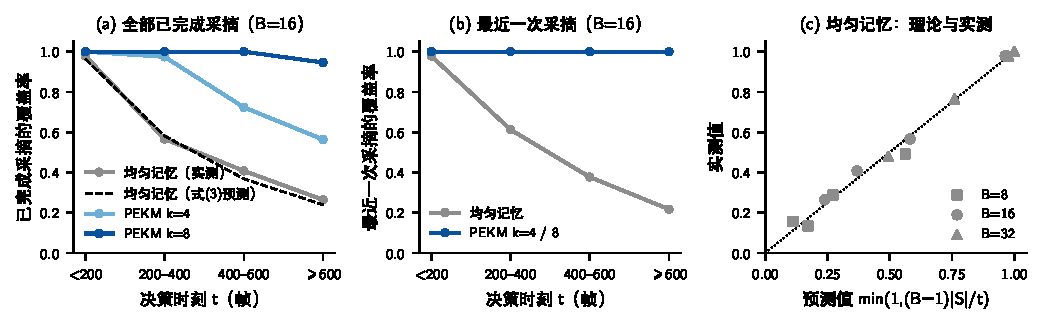
\includegraphics[width=\linewidth]{zh_coverage_theory}
\caption{按时间组织的记忆作业越久忘得越多（真实数据）。(a) $B=16$ 时全部已完成采摘的覆盖率随决策时刻的变化；(b) 最近一次采摘的覆盖率；(c) 各预算与各时间段上均匀记忆覆盖率的理论预测与实测。}
\label{fig:theory}
\end{figure}

\subsection{采摘事件检测（RQ2）}
\label{sec:res_events}
\textbf{几何事件在专家示范上精确，但在闭环中失效。}由真值距离得到的几何事件在专家示范上与真实采摘完全一致：半径在 1--4~cm 之间时，训练集和验证集上的精确率、召回率和 F1 均为 \V{evt_f1_plateau}（图~\ref{fig:events}(a)）。对距离噪声的分析给出了感知模块的精度要求：使用迟滞检测时，\V{spec_white}~cm 白噪声下 F1 为 \V{spec_white_f1}，2~cm 相关噪声下为 \V{spec_ou_f1}；而不加滤波的阈值检测在 1~cm 白噪声下 F1 即降到 \V{white1_plain_f1}，只有 \pct{white1_plain_cnt} 的回合计数正确（图~\ref{fig:events}(b)）。然而，在包含策略闭环回放的评测集上（\V{det_n_ep} 个回合，\V{det_n_ev} 次真实采摘，\V{det_n_fail} 次失败尝试），几何事件把每一次失败尝试都计为采摘，精确率降到 \V{det_geo_p}，只有 \pct{det_geo_cnt} 的回合计数正确（表~\ref{tab:detect}）。

\textbf{\pedet{} 准确、可区分成功与失败，且对光照鲁棒。}\pedet{} 的事件 F1 为 \V{det_pe_f1}，\pct{det_pe_cnt} 的回合计数正确，只有 \pct{det_pe_fp} 的失败尝试被误计为采摘；接触关键帧误差的中位数为 \V{det_pe_tc} 帧，脱离关键帧为 \V{det_pe_tr} 帧（P90 为 \V{det_pe_tr90} 帧），K8 记忆的关键帧召回率为 \V{det_pe_kf}。手工链路 \fdm{} 在标称光照下表现良好（F1 \V{det_fdm_f1}），但它依赖颜色阈值生成提示，光照扰动下 F1 降到 \V{det_fdm_light}（图~\ref{fig:events}(c)）；这与分割实验的结论一致：给定正确的提示框时 SAM 在光照变化下 F1 仍为 \V{samgt_light_f1}，失效的是颜色提示。只用夹爪开度停滞的启发式不受光照影响，但无法区分夹住果实与夹住枝叶、滑脱等情况，失败尝试误报率为 \pct{det_grip_fp}。

\textbf{两种模态互补。}只用视觉时 \pedet{} 已明显优于启发式方法（F1 \V{det_pv_f1}），但在腕部画面被果实或叶片大面积遮挡时会漏检；只用本体感知时 F1 为 \V{det_pp_f1}，对“夹住但未脱离”与“已脱离”的区分较差。两者融合后误报率降到 \pct{det_pe_fp}，说明视觉提供“夹住的是不是果实、果实是否离开果柄”，本体感知提供“夹爪何时闭合、受力如何变化”。

\begin{table}[t]
\centering
\caption{采摘事件检测（仿真 v2 验证集，含专家示范与闭环回放）}
\label{tab:detect}
\small
\setlength{\tabcolsep}{4.5pt}
\begin{tabular}{lcccccc}
\toprule
检测器 & 精确率 & 召回率 & F1 & 计数正确（\%） & 失败尝试误报（\%） & 光照扰动 F1\\
\midrule
几何事件（真值距离，特权） & \V{det_geo_p} & \V{det_geo_r} & \V{det_geo_f1} & \V{det_geo_cnt} & \V{det_geo_fp} & \V{det_geo_light}\\
\fdm{}（手工感知链路） & \V{det_fdm_p} & \V{det_fdm_r} & \V{det_fdm_f1} & \V{det_fdm_cnt} & \V{det_fdm_fp} & \V{det_fdm_light}\\
夹爪停滞启发式 & \V{det_grip_p} & \V{det_grip_r} & \V{det_grip_f1} & \V{det_grip_cnt} & \V{det_grip_fp} & \V{det_grip_light}\\
\pedet{}（仅视觉） & \V{det_pv_p} & \V{det_pv_r} & \V{det_pv_f1} & \V{det_pv_cnt} & \V{det_pv_fp} & \V{det_pv_light}\\
\pedet{}（仅本体） & \V{det_pp_p} & \V{det_pp_r} & \V{det_pp_f1} & \V{det_pp_cnt} & \V{det_pp_fp} & \V{det_pp_light}\\
\textbf{\pedet{}（完整）} & \textbf{\V{det_pe_p}} & \textbf{\V{det_pe_r}} & \textbf{\V{det_pe_f1}} & \textbf{\V{det_pe_cnt}} & \textbf{\V{det_pe_fp}} & \textbf{\V{det_pe_light}}\\
\bottomrule
\end{tabular}
\end{table}

\begin{figure}[t]
\centering
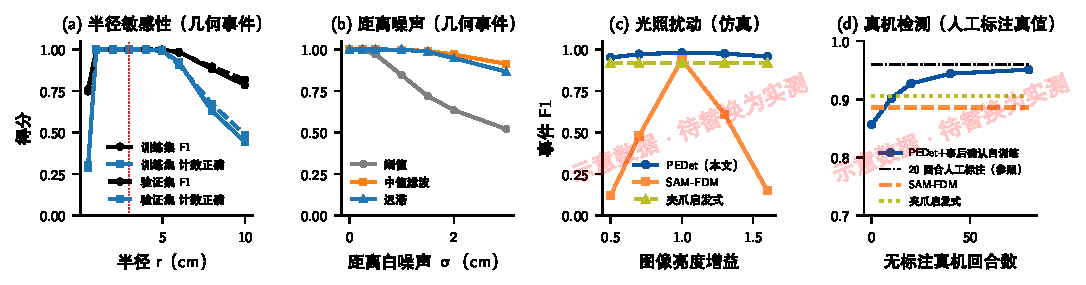
\includegraphics[width=\linewidth]{zh_event_detection}
\caption{事件检测。(a) 几何事件的 F1 与计数正确率随半径 $r$ 的变化（真实）；(b) 几何事件在距离白噪声下的 F1，比较阈值、中值滤波与迟滞三种检测（真实）；(c) 图像亮度增益扰动下三种检测器的事件 F1；(d) 真机上事件 F1 随无标注回合数的变化（事后确认自训练），真值为第三视角人工标注，点划线为 20 个人工标注回合的有监督参照。}
\label{fig:events}
\end{figure}

\subsection{仿真闭环主结果（RQ3）}
\label{sec:res_closed}
\textbf{正对照确认任务都在检验记忆。}在推理时只给 K0 保留最近 16 帧，计数 v2 的记忆类失败率从 \pct{pc_cnt_a} 升到 \pct{pc_cnt_b}（\V{pc_cnt_d}~\pp，95\% CI \V{pc_cnt_ci}），遮挡 v2 从 \pct{pc_occ_a} 升到 \pct{pc_occ_b}（\V{pc_occ_d}~\pp，CI \V{pc_occ_ci}），均远超预设的 15~\pp{} 门槛。与 v1 不同，v2 任务的成败确实取决于长程记忆。

\textbf{HarvestMem 大幅提高了事件记忆任务的成功率。}表~\ref{tab:closed} 与图~\ref{fig:simmain}(a) 给出主结果。在计数 v2 上，K0 的成功率为 \pct{c_k0_s}，HEM 达到 \pct{c_hem_s}，提高 \V{c_dh}~\pp（95\% CI \V{c_dh_ci}，Holm $p$ \V{c_dh_p}），主假设 H1 获得支持；平均计数误差 $|\text{入篮数}-N|$ 从 \V{c_k0_err} 颗降到 \V{c_hem_err} 颗。平坦关键帧同样有效（K4 \V{c_d4}~\pp，K8 \V{c_d8}~\pp），说明“按事件组织记忆”本身是增益的主要来源；HEM 相对 K8 再提高 \V{c_dh8}~\pp（CI \V{c_dh8_ci}），差距较小，与事先预测一致：计数 v2 的配额 $N\le5$ 基本在 K8 的容量之内。关闭安全包络后，HEM$-$K0 为 \V{c_dh_noguard}~\pp（CI \V{c_dh_noguard_ci}），结论不依赖包络；各条件的包络裁剪率接近（约 \pct{c_clip}）。

\textbf{场景记忆任务上各条件等效，与事先预测一致。}在遮挡 v2 上，K0、K4、K8 与 HEM 的成功率分别为 \pct{o_k0_s}、\pct{o_k4_s}、\pct{o_k8_s} 和 \pct{o_hem_s}；HEM$-$K0 为 \V{o_dh}~\pp（CI \V{o_dh_ci}），TOST 检验在 $\pm10$~\pp{} 等效界内成立（$p=\V{o_dh_tost}$）。这一“预测中的无差异”同样重要：它表明 HarvestMem 的增益只出现在信息以事件形式存在的场合，而为事件分配位置并没有挤掉阵风前的关键画面，因为场景锚层始终保留第 0 帧。

\textbf{增益随配额增大，且越接近平坦方案的容量上限，分层的优势越明显。}如图~\ref{fig:simmain}，HEM 相对 K0 的增益在 $N=2$、3、4--5 时分别为 \V{cN_gain_h0.1}、\V{cN_gain_h0.2} 和 \V{cN_gain_h0.3}~\pp；相对 K8 的增益分别为 \V{cN_gain_h8.1}、\V{cN_gain_h8.2} 和 \V{cN_gain_h8.3}~\pp，在 $N=5$ 超过 K8 的 4 次容量时开始显现。配额越大，回合越长、事件越多，均匀记忆按命题~\ref{prop:uniform} 丢失得越多。

\begin{table}[t]
\centering
\caption{仿真闭环结果（val 150--199 $\times$ 种子 7/8/9，每格 \V{n_val} 次；差值单位为百分点，方括号为 95\% CI）}
\label{tab:closed}
\small
\setlength{\tabcolsep}{2.6pt}
\begin{tabular}{llcccccc}
\toprule
任务 & 记忆 & \shortstack{成功率\\（\%）} & \shortstack{记忆类\\失败（\%）} & \shortstack{操作类\\失败（\%）} & \shortstack{计数误差\\（颗）} & $\Delta$ vs K0 & $\Delta$ vs K8\\
\midrule
\multirow{4}{*}{\shortstack{计数 v2\\（事件记忆）}} & K0 均匀 & \V{c_k0_s} & \V{c_k0_mem} & \V{c_k0_op} & \V{c_k0_err} & -- & --\\
 & K4 平坦 & \V{c_k4_s} & \V{c_k4_mem} & \V{c_k4_op} & \V{c_k4_err} & \V{c_d4} \V{c_d4_ci} & --\\
 & K8 平坦 & \V{c_k8_s} & \V{c_k8_mem} & \V{c_k8_op} & \V{c_k8_err} & \V{c_d8} \V{c_d8_ci} & --\\
 & \textbf{HEM} & \textbf{\V{c_hem_s}} & \textbf{\V{c_hem_mem}} & \V{c_hem_op} & \textbf{\V{c_hem_err}} & \textbf{\V{c_dh}} \V{c_dh_ci}\textsuperscript{H1} & \V{c_dh8} \V{c_dh8_ci}\\
\midrule
\multirow{4}{*}{\shortstack{遮挡 v2\\（场景记忆）}} & K0 均匀 & \V{o_k0_s} & \V{o_k0_mem} & -- & -- & -- & --\\
 & K4 平坦 & \V{o_k4_s} & \V{o_k4_mem} & -- & -- & \V{o_d4} \V{o_d4_ci} & --\\
 & K8 平坦 & \V{o_k8_s} & \V{o_k8_mem} & -- & -- & \V{o_d8} \V{o_d8_ci} & --\\
 & HEM & \V{o_hem_s} & \V{o_hem_mem} & -- & -- & \V{o_dh} \V{o_dh_ci}\textsuperscript{T} & --\\
\midrule
\multirow{3}{*}{\shortstack{FruitRow\\（长时事件）}} & K0 均匀 & \V{l_k0_s} & \V{l_k0_mem} & \V{l_k0_op} & \V{l_err_k0} & -- & --\\
 & K8 平坦 & \V{l_k8_s} & \V{l_k8_mem} & \V{l_k8_op} & \V{l_err_k8} & -- & --\\
 & \textbf{HEM} & \textbf{\V{l_hem_s}} & \textbf{\V{l_hem_mem}} & \V{l_hem_op} & \textbf{\V{l_err_hem}} & \textbf{\V{l_dh0}} \V{l_dh0_ci}\textsuperscript{H2} & \textbf{\V{l_dh8}} \V{l_dh8_ci}\textsuperscript{H3}\\
\bottomrule
\end{tabular}

\vspace{2pt}
{\footnotesize H1--H3：预登记主假设，Holm 校正后 $p$ 均 \V{l_p}。T：TOST 等效检验 $p=\V{o_dh_tost}$（$\pm10$~\pp）。}
\end{table}

\begin{figure}[t]
\centering
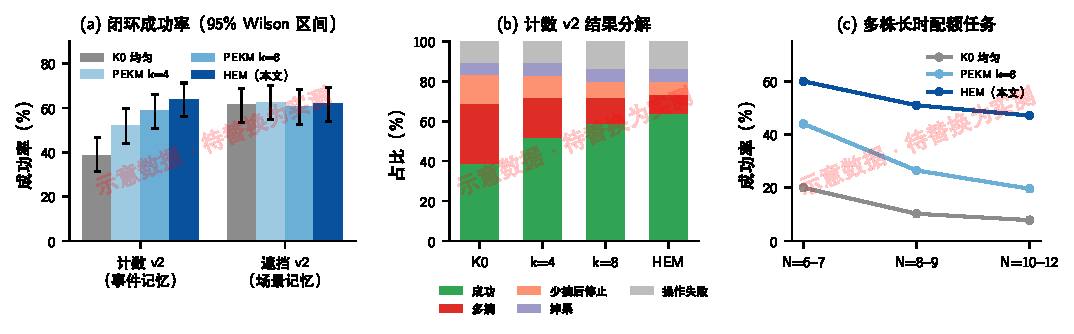
\includegraphics[width=\linewidth]{zh_sim_main}
\caption{仿真闭环结果。(a) 计数 v2 与遮挡 v2 上四种记忆的成功率；(b) 计数 v2 的结果分解，增益几乎全部来自多摘和少摘后停止这两类记忆失败的减少；(c) FruitRow 按配额 $N$ 分层的成功率，平坦关键帧在采摘次数超出其容量后迅速下降。}
\label{fig:simmain}
\end{figure}

\subsection{长时作业中的可扩展性（RQ4）}
\label{sec:res_long}
\textbf{分层记忆在长时作业中优势最大。}FruitRow 平均每回合 \V{row_events} 次采摘，远超平坦关键帧的容量。如表~\ref{tab:closed}，K0 的成功率只有 \pct{l_k0_s}，K8 为 \pct{l_k8_s}，HEM 达到 \pct{l_hem_s}：相对 K0 提高 \V{l_dh0}~\pp（CI \V{l_dh0_ci}），相对 K8 提高 \V{l_dh8}~\pp（CI \V{l_dh8_ci}），主假设 H2、H3 均获支持（Holm $p$ \V{l_p}）。平均计数误差从 K0 的 \V{l_err_k0} 颗、K8 的 \V{l_err_k8} 颗降到 \V{l_err_hem} 颗。

\textbf{性能随配额的变化与容量分析吻合。}如图~\ref{fig:simmain}(c)，当 $N$ 从 6--7 增加到 10--12，K8 的成功率从 \pct{lN_k8.1} 降到 \pct{lN_k8.3}，与它约 4 次的容量一致：更早的采摘只能依靠时间上下文层碰运气。HEM 只从 \pct{lN_hem.1} 缓降到 \pct{lN_hem.3}，下降主要来自回合变长后操作失败的累积，而不是记忆失败。这是命题~\ref{prop:capacity} 在闭环中的直接体现。

\textbf{分层结构的每个部分都必要。}表~\ref{tab:ablation}(b) 在 FruitRow 上逐一去除 \hem{} 的组件。去掉情景摘要层后，\hem{} 只保留最近 2 次采摘，成功率降到 \pct{al_nosum}，低于 K8；摘要层用单帧代替拼图（容量 5 次）时为 \pct{al_single}；改用 $3\times3$ 拼图虽把容量提高到 29 次，但每格分辨率降低、且本任务的采摘次数已在 $2\times2$ 拼图的容量之内，成功率为 \pct{al_mosaic9}，略低于默认设置。去掉类型-时间嵌入后成功率降到 \pct{al_noemb}：策略无法区分拼图帧与普通帧，也无法判断事件的先后。去掉事件扰动训练后为 \pct{al_noept}。

\subsection{增益从何而来：机制与消融（RQ5）}
\label{sec:res_ablation}
\textbf{增益来自记忆类失败的减少。}如图~\ref{fig:simmain}(b)，从 K0 到 HEM，计数 v2 的记忆类失败率从 \pct{c_k0_mem} 降到 \pct{c_hem_mem}，而操作类失败率基本不变（\pct{c_k0_op} 与 \pct{c_hem_op}）。增益集中在“多摘”上，这正是记住自己每次放果所能避免的错误。

\textbf{反事实对照排除了“换帧扰动”的解释。}表~\ref{tab:ablation}(a) 中，若保留同样数量的事件位置，但把关键帧整体错后 24 帧（不再对准接触与脱离），成功率降到 \pct{ab_shift}；若事件位置随机选取，则为 \pct{ab_random}，均与 K0 相当。改变记忆的\emph{内容}而非\emph{位置数量}才带来增益。只保留接触帧时成功率为 \pct{ab_contact}，只保留脱离帧时为 \pct{ab_release}：脱离帧显示“果实已离开果柄、正被带走”，直接对应“又摘了一颗”。

\textbf{学习型检测接近物理真值，且优于特权几何信号。}使用仿真物理事件（上界）时成功率为 \pct{ab_oracle}，\pedet{} 为 \pct{ab_pedet}，仅差 \V{ab_gap}~\pp；使用真值距离的几何事件反而降到 \pct{ab_geo}，因为闭环中的失败尝试被当作采摘写入记忆；\fdm{} 和夹爪启发式分别为 \pct{ab_fdm} 和 \pct{ab_grip}。光照扰动下，HEM+\pedet{} 保持在 \pct{ab_light_pedet}，HEM+\fdm{} 降到 \pct{ab_light_fdm}，与同样条件下的 K0（\pct{ab_light_k0}）相差无几：事件丢失时 \hem{} 自动退化为均匀记忆，而不会比均匀记忆更差。

\textbf{事件扰动训练使策略对检测误差鲁棒。}去掉 EPT 重新训练后，计数 v2 成功率从 \pct{ab_pedet} 降到 \pct{ab_noept}。在推理时人为注入 10\% 漏检，有 EPT 的策略为 \pct{ab_noise_ept}，几乎不受影响；无 EPT 的策略降到 \pct{ab_noise_noept}，多摘明显增加，说明未经扰动训练的策略会无条件信任记忆。直接在推理时给 K0 策略换上 \hem{} 记忆（训练中从未见过），成功率为 \pct{ab_untrained}，不优于 K0：训练与部署必须使用同一记忆构造函数。

\begin{table}[t]
\centering
\caption{消融与反事实对照（每项 150 次）}
\label{tab:ablation}
\small
\begin{tabular}{llc}
\toprule
因素 & 设置 & 成功率（\%）\\
\midrule
\multicolumn{3}{l}{\textbf{(a) 计数 v2，HEM 策略}}\\
默认 & HEM + \pedet{} + EPT & \textbf{\V{ab_pedet}}\\
\multirow{4}{*}{事件来源} & 仿真物理事件（上界） & \V{ab_oracle}\\
 & 几何事件（真值距离，特权） & \V{ab_geo}\\
 & \fdm{} & \V{ab_fdm}\\
 & 夹爪停滞启发式 & \V{ab_grip}\\
\multirow{3}{*}{光照扰动} & K0 均匀 & \V{ab_light_k0}\\
 & HEM + \fdm{} & \V{ab_light_fdm}\\
 & HEM + \pedet{} & \V{ab_light_pedet}\\
\multirow{2}{*}{反事实} & 关键帧错后 24 帧（位置数相同） & \V{ab_shift}\\
 & 事件位置随机选取 & \V{ab_random}\\
\multirow{2}{*}{关键帧组成} & 只保留接触帧 & \V{ab_contact}\\
 & 只保留脱离帧 & \V{ab_release}\\
\multirow{3}{*}{鲁棒训练} & 去掉 EPT（重新训练） & \V{ab_noept}\\
 & 注入 10\% 漏检：有 EPT / 无 EPT & \V{ab_noise_ept} / \V{ab_noise_noept}\\
 & K0 策略推理时改用 \hem{}（训练未见） & \V{ab_untrained}\\
\midrule
\multicolumn{3}{l}{\textbf{(b) FruitRow，HEM 结构（均重新训练）}}\\
默认 & 完整 \hem{}（$2\times2$ 拼图，容量 \V{cap_hem}） & \textbf{\V{al_full}}\\
\multirow{5}{*}{结构} & 去掉情景摘要层（容量 2） & \V{al_nosum}\\
 & 摘要层用单帧代替拼图（容量 5） & \V{al_single}\\
 & $3\times3$ 拼图（容量 29，单格分辨率更低） & \V{al_mosaic9}\\
 & 去掉类型-时间嵌入 & \V{al_noemb}\\
 & 去掉事件扰动训练 & \V{al_noept}\\
\bottomrule
\end{tabular}
\end{table}

\subsection{真实番茄采摘实验（RQ6）}
\label{sec:res_real}
\textbf{事后确认自训练无需人工标注即可完成检测器迁移。}在 \V{rb_det_ep} 个独立真机回合（\V{rb_det_ev} 次真实采摘）上，以第三视角人工标注为真值（表~\ref{tab:realdet}），仅在仿真中训练的 \pedet{} 的 F1 为 \V{rd_zero.3}，低于夹爪启发式（\V{rd_grip.3}），主要误差来自真实番茄的颜色与反光差异。经过 \V{rb_hsl_ep} 个无标注回合的事后确认自训练，F1 提高到 \V{rd_hsl.3}，与用 \V{rb_sup_ep} 个人工标注回合有监督微调的参照（\V{rd_sup.3}）几乎相当，脱离关键帧误差中位数为 \V{rd_tr} 帧。\pct{hsl_keep} 的持物段通过一致性筛选，伪标签的事件精确率为 \V{hsl_prec}。图~\ref{fig:events}(d) 显示，10 个无标注回合就足以超过两种基线。\fdm{} 在真机上受果皮反光造成的深度空洞和光照影响，F1 为 \V{rd_fdm.3}。

\textbf{真机闭环结果与仿真一致。}如图~\ref{fig:real} 与表~\ref{tab:real}，在真机计数任务上，HEM 的成功率为 \pct{rc_hem_s}，K0 为 \pct{rc_k0_s}（\V{rc_d}~\pp，配对符号翻转检验 $p=\V{rc_p}$），平均计数误差从 \V{rc_err_k0} 颗降到 \V{rc_err_hem} 颗；增益主要来自多摘的减少（K0 \V{rc_k0.2} 次，HEM \V{rc_hem.2} 次）。HEM 相对 K8（\pct{rc_k8_s}）高 \V{rc_d8}~\pp（$p=\V{rc_p8}$），真机配额 $N\le3$ 在 K8 容量之内，这一差距与仿真中计数 v2 的结果一致。在真机遮挡任务上，K0 与 HEM 分别为 \pct{ro_k0_s} 和 \pct{ro_hem_s}，符合“场景记忆无差异”的预测。在暖色光照扰动下，HEM+\pedet{} 的计数任务成功率为 \pct{rl_pedet_s}，HEM+\fdm{} 降到 \pct{rl_fdm_s}。在日光温室的盆栽番茄上，HEM 完成 \V{gh_hem} 次、K0 完成 \V{gh_k0} 次。单回合平均用时 K0 为 \V{rt_k0}~s，HEM 为 \V{rt_hem}~s，两者相当。

\begin{table}[t]
\centering
\caption{真机结果。上：采摘事件检测（\V{rb_det_ep} 回合，第三视角人工标注真值）；下：闭环结果（每条件 \V{rb_trials} 次）}
\label{tab:realdet}
\label{tab:real}
\small
\begin{tabular}{lccc}
\toprule
检测器 & 精确率 & 召回率 & F1\\
\midrule
夹爪停滞启发式 & \V{rd_grip.1} & \V{rd_grip.2} & \V{rd_grip.3}\\
\fdm{} & \V{rd_fdm.1} & \V{rd_fdm.2} & \V{rd_fdm.3}\\
\pedet{}（仅仿真训练） & \V{rd_zero.1} & \V{rd_zero.2} & \V{rd_zero.3}\\
\textbf{\pedet{} + 事后确认自训练（零标注）} & \textbf{\V{rd_hsl.1}} & \textbf{\V{rd_hsl.2}} & \textbf{\V{rd_hsl.3}}\\
\pedet{} + \V{rb_sup_ep} 回合人工标注（参照） & \V{rd_sup.1} & \V{rd_sup.2} & \V{rd_sup.3}\\
\midrule
闭环条件 & 成功率（\%） & 多摘 / 少摘停止 & 掉果 / 操作失败\\
\midrule
真机计数：K0 均匀 & \V{rc_k0_s} & \V{rc_k0.2} / \V{rc_k0.3} & \V{rc_k0.4} / \V{rc_k0.5}\\
真机计数：K8 平坦 & \V{rc_k8_s} & \V{rc_k8.2} / \V{rc_k8.3} & \V{rc_k8.4} / \V{rc_k8.5}\\
真机计数：\textbf{HEM} & \textbf{\V{rc_hem_s}} & \V{rc_hem.2} / \V{rc_hem.3} & \V{rc_hem.4} / \V{rc_hem.5}\\
真机遮挡：K0 / HEM & \V{ro_k0_s} / \V{ro_hem_s} & -- & --\\
暖光计数：HEM+\fdm{} / HEM+\pedet{} & \V{rl_fdm_s} / \V{rl_pedet_s} & -- & --\\
温室番茄：K0 / HEM（成功次数） & \V{gh_k0} / \V{gh_hem} & -- & --\\
\bottomrule
\end{tabular}
\end{table}

\begin{figure}[t]
\centering
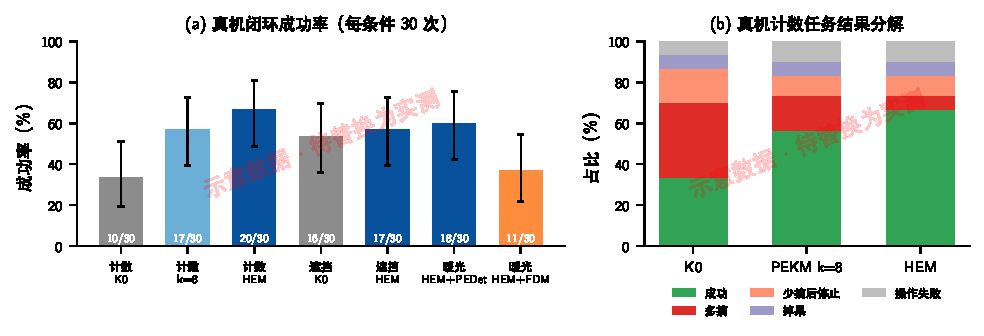
\includegraphics[width=0.92\linewidth]{zh_real}
\caption{真机闭环结果。(a) 各条件成功率与 Wilson 95\% 区间；(b) 真机计数任务的结果分解。}
\label{fig:real}
\end{figure}

\subsection{记忆内容对 VLA 策略的影响（补充证据）}
\label{sec:res_general}
本文的前提是：固定预算记忆的\emph{内容}会影响 VLA 策略的行为。我们在一个通用操作记忆基准上，以相同结构的基础策略、在封存协议和配对检验下验证了这一点（真实结果）：去掉历史记忆后，模式回忆任务成功率从 \pct{robomme_nomem_a} 降到 \pct{robomme_nomem_b}（$-65.0$~\pp，95\% CI $[-81.7,-46.7]$，$p<0.001$）；记忆预算从 32 帧减半到 16 帧，成功率从 \pct{robomme_half_a} 降到 \pct{robomme_half_b}（$-37.8$~\pp，$p<0.001$）；替换单个记忆位置会改变动作损失，位置重要性排序的可靠度在四个任务上为 0.97--0.99。也就是说，在固定预算内记住什么确实重要，而这正是 HarvestMem 利用采摘的物理结构所做的决定。

\subsection{运行开销}
\label{sec:res_cost}
表~\ref{tab:cost} 汇总了各组件的开销。\hem{} 构造一次记忆耗时约 \V{hem_ms}~ms，拼图帧只在有事件进入摘要层时编码一次；由于记忆图像数和 token 数不变，策略的显存与推理开销与均匀记忆完全相同，新增参数仅约 \V{hem_params}~M。\pedet{} 每帧耗时 \V{pedet_ms}~ms，可与控制循环并行运行。作为对比，\fdm{} 需在每回合开始时运行一次 SAM（ViT-B \V{sam_ms_b}~ms，ViT-H \V{sam_ms_h}~ms），并依赖深度相机与精确外参。

\begin{table}[t]
\centering
\caption{运行开销（仿真：NVIDIA L20；真机：\V{rb_gpu}）}
\label{tab:cost}
\small
\begin{tabular}{lll}
\toprule
组件 & 开销 & 频率\\
\midrule
均匀采样 / 平坦关键帧选帧（$t=1000$） & \V{unif_us} / \V{pekm_us}~$\mu$s（CPU 单核） & 每次决策\\
\hem{} 记忆构造（含拼图） & \V{hem_ms}~ms（CPU） & 每次决策\\
类型-时间嵌入 & 新增约 \V{hem_params}~M 参数，计算可忽略 & 每次决策\\
\pedet{} & 仿真 \V{pedet_ms}~ms；真机 \V{rt_pedet}~ms & 每控制步\\
VLA 推理（一个动作块） & 仿真 \V{sim_vla_ms}~ms；真机 \V{rt_vla}~ms & 每 16 步\\
\fdm{} 的 SAM 分割 & ViT-B \V{sam_ms_b}~ms；ViT-H \V{sam_ms_h}~ms & 每回合一次\\
\bottomrule
\end{tabular}
\end{table}

\section{讨论}
\label{sec:discussion}

\textbf{从通用 VLA 到农业特需 VLA。}本文的结果表明，通用 VLA 在桌面任务上形成的记忆设计（固定帧数、按时间均匀采样）在农业长时作业中存在结构性缺陷，而且这一缺陷无法通过调参或适度扩大预算消除。农业场景真正需要的不是“记更多帧”，而是“记对的东西”：场景锚保住被遮挡之前的画面，工作事件层保住刚刚发生的细节，摘要层以极低的代价保住整行作业的进度。HarvestMem 只替换了通用结构中“记什么、怎么组织”这一环节，其余部分原样沿用，因此可以直接嫁接到不同的 VLA 骨干上，并随通用模型的进步而进步。我们认为，这种“通用骨干 + 领域特需记忆”的范式，是把大模型能力落地到农业装备的一条可行路径。

\textbf{对农业作业的意义。}按配额采收、分级抽样、疏果和按订单采摘，本质上都要求机器人记住自己做过什么；在枝叶茂密的冠层中，“曾经看见过什么”同样需要被记住。HarvestMem 不改变基础模型的记忆帧数和推理开销，新增参数仅约 \V{hem_params}~M，\pedet{} 是可与控制循环并行的轻量网络，事后确认自训练只依赖夹爪和腕部相机这两种所有采摘机器人都具备的传感器。对算力受限、难以人工标注的田间平台，这比扩大记忆预算、引入大型记忆模块或在植株上布设传感器都更容易落地。

\textbf{为什么“无差异”也是重要结果。}遮挡 v2 上各记忆条件等效，并不说明方法失效，而是确认了它的作用边界：场景信息集中在开头画面中，均匀采样与场景锚层都会保留它；\hem{} 只改变事件型信息的保留方式，并且没有挤掉开头画面。正因为两类任务的预测在评测前就已写定，事件记忆任务上的增益才更可信，而不是事后挑出的有利结果。同理，计数 v2 上 HEM 与 K8 的差距较小、FruitRow 上差距显著，也都与容量分析的事先预测一致。

\textbf{基准设计的教训。}v1 的经验表明，按直觉设计的“记忆任务”很可能存在捷径：环境的终止逻辑、遮挡物的物理交互、甚至成熟度的先验比例，都可能让策略绕开记忆。我们建议，任何声称检验记忆的机器人基准都应报告信息受限脚本策略的审计结果，并设置正对照。这一做法成本很低，却能决定实验结论是否有意义。

\textbf{为什么需要学习型检测器与事后确认。}几何距离只描述“靠近了果实”，而采摘任务关心的是“果实是否真的被摘下”；手工感知链路证明了“从感知中恢复事件”是可行的，也暴露了它对颜色提示和光照的依赖。\pedet{} 把检测目标从几何量换成物理结果，使闭环中常见的失败尝试不再污染记忆。事后确认自训练进一步解决了真机标签的来源问题：采摘的成败在果实入篮时才可确认，确认后回溯标注事件时刻，既不需要人工标注，也不需要在果实上安装任何装置，检测器因此可以随作物、季节和光照的变化持续更新。

\textbf{局限。}第一，仿真中的果实为刚体球，果柄约束经过简化，真实果实的形变、果柄柔性和成簇生长尚未建模。第二，真机主实验采用“真实番茄 + 可复位植株骨架”，以换取可重复的配对比较，与温室和果园中的枝叶柔性、自然风扰和光照变化仍有差距；温室验证规模较小，不做配对检验；用窄带照明模拟“颜色不可分”也只是场景记忆需求的一种实验室近似。第三，事件定义针对“夹持—拉拽”式采摘，剪切式末端执行器需要把“剪刀闭合”纳入事件定义；事后确认依赖“入篮”这一结果，若采用传送带或吸管式收集，需要相应修改确认规则。第四，拼图帧以较低分辨率保存远期事件，若任务需要回忆远期事件的细节（如某颗果的确切成熟度），摘要层可能不够用。第五，真机每条件 \V{rb_trials} 次试验只能检测较大的效应，较小的差异需要更大规模的田间验证。

\textbf{未来工作。}下一步计划在温室番茄和果园苹果上开展移动平台的整行连续作业试验，将事件语义扩展到放果确认、掉果检测、剪梗与抓取重试，并研究把事件记忆与三维场景记忆结合，使机器人同时记住“哪里有什么”和“自己做过什么”。

\section{结论}
\label{sec:conclusion}
本文面向农业长时采摘作业，研究了 VLA 模型在固定记忆预算下“记什么、怎么组织”的问题。理论分析和实测表明，通用 VLA 按时间均匀采样的记忆对短暂采摘事件的覆盖率随作业时长按 $1/t$ 衰减，16 帧记忆平均只记得约 \V{cap_u} 次采摘。为此提出事件中心分层记忆 VLA 模型 HarvestMem，包含三项创新：物理监督的学习型采摘事件检测器 \pedet，零人工标注训练，能区分成功采摘与失败尝试并对光照鲁棒；事件中心分层记忆 \hem，以场景锚、工作事件、情景摘要拼图帧和时间上下文组织固定预算，并以类型-时间嵌入编码记忆语义，在不增加推理开销的前提下把可保留的采摘次数提升到 \V{cap_hem} 次；事件扰动训练与事后确认自训练，使策略对检测误差鲁棒，并使检测器无需人工标注、无需附加传感器即可适配真机。在经过捷径审计的 \bench{} 基准上，HarvestMem 把事件记忆计数任务成功率从 \pct{c_k0_s} 提高到 \pct{c_hem_s}，把多株长时配额任务从 \pct{l_k0_s} 提高到 \pct{l_hem_s}，在场景记忆任务上与均匀记忆等效，与事先预测一致；真实番茄计数任务成功率从 \pct{rc_k0_s} 提高到 \pct{rc_hem_s}。按物理事件组织记忆，为通用 VLA 走向农业长时作业提供了一条简单、可审计且易于部署的途径。


\vspace{0.6em}
\noindent{\heiti 基金项目：}\V{fund}

\noindent{\heiti 数据与代码：}仿真基准、训练配置、预登记协议与评测脚本将在论文接收后公开 \todo{仓库地址}。

{\small\linespread{1.08}\selectfont
\setlength{\bibsep}{1pt plus 0.5pt}
\bibliographystyle{gbt7714-numerical}
\bibliography{references}
}

\ifshownotes
\clearpage
\appendix
\section*{附录 A\quad 写作说明与待替换清单（投稿前删除）}
\addcontentsline{toc}{section}{附录 A 写作说明与待替换清单}
\markboth{附录 A\quad 写作说明}{附录 A\quad 写作说明}
\small

\subsection*{A.1 数值的三种状态}
全部数值集中在 \texttt{data/values.yaml}，每项为 \texttt{[值, 状态, 来源]}。\texttt{real}（\NumReal{} 项）来自已有运行，正常显示；\texttt{ideal}（\NumIdeal{} 项）为理想示意值，正文中显示为\textcolor{red}{红色}，相关图片带“示意数据”水印；\texttt{todo}（\NumTodo{} 项）为待确认信息，显示为\textcolor{orange!85!black}{[橙色方括号]}。实验完成后，把实测值填入对应项并把状态改为 \texttt{real}，运行 \texttt{./build.sh} 即可同步更新正文、表格和图片。表~\ref{tab:coverage} 和第~\ref{sec:res_general} 节的数字是真实结果，直接引自英文稿 v0.4（\texttt{paper/results/memory\_coverage.json} 与 RoboMME 评测），未经 \texttt{values.yaml}。

\textbf{示意值不是预测。}示意值是按“实验取得预期结果”设定的、内部自洽的数字（例如失败分类之和等于总次数，分层成功率与总成功率一致），只用于搭建叙事。实测结果的方向或大小与示意值不同时，不仅要改数字，还要改依赖结论方向的句子，主要在：摘要与引言贡献列表的结果句；第~\ref{sec:res_closed}、\ref{sec:res_long} 节各段的小标题和首句；第~\ref{sec:res_ablation} 节“事件来源”“事件扰动训练”两段；第~\ref{sec:res_real} 节；结论。图~\ref{fig:capacity} 与第~\ref{sec:coverage}、\ref{sec:hem} 节的容量数字（约 \V{cap_u}、约 \V{cap_k8}、\V{cap_hem}、\V{cap_flat_max}）是按设计参数真实计算的，由 \texttt{tools/make\_figures\_zh.py} 中的 \texttt{fig\_capacity} 生成；改动 $m_w$、$c$、$s_{\max}$ 后需重新运行。

\subsection*{A.2 尚待实现与完成的实验（对应章节）}
\begin{enumerate}
\item \textbf{R0 捷径审计}（表~\ref{tab:audit}）：交接文档修订 7 第 15.4 节，正在执行；FruitRow 一行需在 R0 之后追加。
\item \textbf{\hem{} 的实现}（第~\ref{sec:hem} 节）：分层选帧函数（含场景锚、自适应分配）、拼图帧构造（脱离后第 3 帧前置图像、以 TCP 投影为中心裁剪 $112\times112$、$2\times2$ 拼接、空格屏蔽）、类型-时间嵌入（零初始化，接到记忆分支 token 上）。训练与部署须调用同一函数；需新增“记忆帧与声明规则一致”的逐决策核验。
\item \textbf{\pedet{} 的实现与训练}（第~\ref{sec:pedet} 节，表~\ref{tab:detect}，图~\ref{fig:events}(c)）：从仿真读取指尖接触与果柄约束生成逐帧标签；采集基础策略在训练布局上的闭环回放；实现域随机化。网络结构与超参数为设计值，按实际实现修改。
\item \textbf{事件扰动训练 EPT}（第~\ref{sec:ept} 节）：在训练样本的记忆构造前对事件表做删除、误插和抖动；扰动率以真机检测误差为准。
\item \textbf{FruitRow 环境}（第~\ref{sec:tasks} 节）：3 株植物、换株信号、整行配额、风落果；专家示范与审计。
\item \textbf{v2 示范、K0/K4/K8/HEM 训练与正式评测}（表~\ref{tab:closed}、图~\ref{fig:simmain}、正对照）：修订 7 第 15.5 节需相应扩展为四个条件和三个任务，主假设族改为 H1--H3；协议须事先写明部署时事件由 \pedet{} 给出、K4/K8 与 HEM 共用 EPT。
\item \textbf{消融}（表~\ref{tab:ablation}）：(a) 为推理期变体，(b) 中各项及“去掉 EPT”需重新训练。
\item \textbf{仿真光照扰动}：渲染亮度增益 0.5--1.6，用于图~\ref{fig:events}(c) 与消融。
\item \textbf{真机实验}（第~\ref{sec:real_design} 节全部）：番茄实验架与弹簧果梗夹（拉脱力标定）、舵机拨杆与叶帘、窄带照明可分性验证、第三视角相机与双人标注流程、遥操作示范、事后确认自训练（持物段阈值、篮区标定、指间区域像素差阈值）、检测评测与闭环评测、温室验证。表~\ref{tab:hardware} 的硬件型号均待确认；图~\ref{fig:realsetup} 待替换为实物照片。
\item \textbf{运行开销}：测量仿真与真机上的 VLA 推理、\pedet{} 和 \hem{} 构造耗时。
\item \textbf{可选}：用 v2 示范重算第~\ref{sec:res_memory} 节的离线覆盖率分析，并加入 \hem{} 一行，使离线与闭环结果来自同一版本的数据。
\end{enumerate}

\subsection*{A.3 需要你决定的事项}
\begin{enumerate}
\item \textbf{方法范围。}\hem{}、拼图帧、类型-时间嵌入、EPT、HSL 和 FruitRow 都是本稿新增的设计，尚未写入交接文档，也未经封存协议。按约定，修改记忆方法与系统定义需要你确认后才能交给执行端实现。
\item \textbf{事件定义。}本稿以“与成熟度无关的物理采摘事件（接触 + 脱离）”为主定义，几何距离事件作为基线。当前代码（\texttt{fruit\_distance.py}）计算的是到“成熟且仍挂树”果实的距离，与本稿不一致。
\item \textbf{基础模型的引用。}正文按要求不突出基础模型的名称，只在第~\ref{sec:base} 节以“当前主流结构”描述并引用 $\pi_0$/$\pi_{0.5}$；记忆分支的结构来源建议仍保留一处引用（第~\ref{sec:related} 节已有），以符合学术规范。
\item \textbf{是否保留 v1 的零结果}（第~\ref{sec:v1} 节与表~\ref{tab:v1}）。这些是真实结果，写成“基准有效性”的动机能增强可信度。
\item \textbf{目标期刊与格式。}本稿按中文期刊常见结构撰写；若投英文期刊，可在定稿后翻译并改用 elsarticle 模板。
\item \textbf{真机规模。}每条件 30 次只能可靠检测约 30~\pp{} 量级的差异，真机 HEM$-$K8 的差距预计不显著；若希望真机上也体现分层优势，需要增加一个真机长时任务（如两株番茄架连续作业）或增加布局数。
\end{enumerate}

\subsection*{A.4 需要核对的参考文献与数字}
\texttt{shi2025memoryvla}、\texttt{fang2025sam2act}、\texttt{kim2024imagegrid} 的作者、题目和出处需要核对；引言中 Bac 等综述的“平均成功率约 66\%、作业周期约 33~s”需对照原文核实；番茄果梗分离力需补充文献。其余文献沿用英文稿 v0.4 的已核对条目，新增的经典文献（RT-1、Q-attention、TCN、域随机化、捷径学习、ResNet、focal loss、伪标签、Noisy Student、HER、bootstrap、Wilson 区间）建议投稿前统一再核一次页码与卷期。

\subsection*{A.5 示意值与待确认信息清单}
{\footnotesize
\begin{longtable}{p{3.2cm}p{0.9cm}p{4.2cm}p{6.2cm}}
\toprule
键名 & 状态 & 当前值 & 说明\\
\midrule
\endhead
\texttt{author1} & todo & 作者一 & \\
\texttt{author2} & todo & 作者二 & \\
\texttt{author3} & todo & 通信作者 & \\
\texttt{affil} & todo & 单位，城市 邮编 & \\
\texttt{email} & todo & email@example.com & \\
\texttt{fund} & todo & 基金项目名称（编号） & \\
\texttt{aud\_cnt\_o1} & ideal & 14 & 计数 v2：仅当前帧脚本策略成功率 \%\\
\texttt{aud\_cnt\_o2} & ideal & 18 & 计数 v2：第 0 帧+当前帧\\
\texttt{aud\_cnt\_o3} & ideal & 96 & 计数 v2：完整历史\\
\texttt{aud\_occ\_o1} & ideal & 26 & 遮挡 v2：仅当前帧\\
\texttt{aud\_occ\_o2} & ideal & 94 & 遮挡 v2：第 0 帧+当前帧\\
\texttt{aud\_occ\_o3} & ideal & 96 & 遮挡 v2：完整历史\\
\texttt{exp\_cnt} & ideal & 93.5 & 计数 v2 专家逐尝试成功率 \%\\
\texttt{exp\_occ} & ideal & 95.0 & 遮挡 v2 专家逐尝试成功率 \%\\
\texttt{clip\_cnt} & ideal & 0.21 & 示范通过安全包络的裁剪率 \%\\
\texttt{clip\_occ} & ideal & 0.18 & \\
\texttt{det\_n\_ep} & ideal & 300 & 检测评测回合数（专家示范 100 + 策略闭环回放 200）\\
\texttt{det\_n\_ev} & ideal & 812 & 真值采摘事件数\\
\texttt{det\_n\_fail} & ideal & 164 & 失败抓取尝试数\\
\texttt{det\_geo\_p} & ideal & 0.832 & \\
\texttt{det\_geo\_r} & ideal & 1.000 & \\
\texttt{det\_geo\_f1} & ideal & 0.908 & \\
\texttt{det\_geo\_cnt} & ideal & 61.3 & 计数正确回合 \%\\
\texttt{det\_geo\_fp} & ideal & 100 & 失败尝试被计为采摘的比例 \%（几何定义下必然）\\
\texttt{det\_geo\_light} & ideal & 1.000 & 光照扰动下 F1（不依赖图像）\\
\texttt{det\_fdm\_p} & ideal & 0.903 & \\
\texttt{det\_fdm\_r} & ideal & 0.981 & \\
\texttt{det\_fdm\_f1} & ideal & 0.940 & \\
\texttt{det\_fdm\_cnt} & ideal & 74.7 & \\
\texttt{det\_fdm\_fp} & ideal & 38 & \\
\texttt{det\_fdm\_light} & ideal & 0.214 & \\
\texttt{det\_grip\_p} & ideal & 0.887 & \\
\texttt{det\_grip\_r} & ideal & 0.952 & \\
\texttt{det\_grip\_f1} & ideal & 0.918 & \\
\texttt{det\_grip\_cnt} & ideal & 66.0 & \\
\texttt{det\_grip\_fp} & ideal & 41 & \\
\texttt{det\_grip\_light} & ideal & 0.918 & \\
\texttt{det\_pv\_p} & ideal & 0.942 & \\
\texttt{det\_pv\_r} & ideal & 0.957 & \\
\texttt{det\_pv\_f1} & ideal & 0.949 & \\
\texttt{det\_pv\_cnt} & ideal & 81.3 & \\
\texttt{det\_pv\_fp} & ideal & 12 & \\
\texttt{det\_pv\_light} & ideal & 0.902 & \\
\texttt{det\_pp\_p} & ideal & 0.901 & \\
\texttt{det\_pp\_r} & ideal & 0.963 & \\
\texttt{det\_pp\_f1} & ideal & 0.931 & \\
\texttt{det\_pp\_cnt} & ideal & 72.0 & \\
\texttt{det\_pp\_fp} & ideal & 33 & \\
\texttt{det\_pp\_light} & ideal & 0.931 & \\
\texttt{det\_pe\_p} & ideal & 0.978 & \\
\texttt{det\_pe\_r} & ideal & 0.983 & \\
\texttt{det\_pe\_f1} & ideal & 0.980 & \\
\texttt{det\_pe\_cnt} & ideal & 92.7 & \\
\texttt{det\_pe\_fp} & ideal & 4 & \\
\texttt{det\_pe\_light} & ideal & 0.962 & \\
\texttt{det\_pe\_tc} & ideal & 1 & 接触关键帧误差中位数（帧）\\
\texttt{det\_pe\_tr} & ideal & 0 & 脱离关键帧误差中位数（帧）\\
\texttt{det\_pe\_tr90} & ideal & 2 & 脱离关键帧误差 P90（帧）\\
\texttt{det\_pe\_kf} & ideal & 0.987 & K8 记忆关键帧召回（±3 帧）\\
\texttt{pedet\_params} & ideal & 1.9 & 时序与融合模块参数量（M），以实际实现为准\\
\texttt{pedet\_ms} & ideal & 1.6 & 检测头单帧延迟 ms（L20）\\
\texttt{fig\_light\_pedet} & ideal & 0.951, 0.972, 0.98, 0.975, 0.958 & \\
\texttt{fig\_light\_fdm} & ideal & 0.12, 0.48, 0.94, 0.61, 0.15 & \\
\texttt{fig\_light\_grip} & ideal & 0.918, 0.918, 0.918, 0.918, 0.918 & \\
\texttt{hem\_params} & ideal & 0.14 & 类型与时间嵌入新增参数（M），按实现修改\\
\texttt{hem\_ms} & ideal & 0.21 & HEM 选帧与拼图构建耗时 ms（CPU）\\
\texttt{fm\_steps} & todo & 10 & 流匹配积分步数，按实际配置确认\\
\texttt{c\_k0} & ideal & 58, 45, 22, 9, 16 & K0 均匀记忆\\
\texttt{c\_k4} & ideal & 78, 30, 16, 10, 16 & 平坦 PEKM k=4\\
\texttt{c\_k8} & ideal & 88, 20, 12, 10, 20 & 平坦 PEKM k=8\\
\texttt{c\_hem} & ideal & 96, 14, 10, 10, 20 & HEM（完整 HarvestMem）\\
\texttt{c\_k0\_s} & ideal & 38.7 & 成功率 \%\\
\texttt{c\_k4\_s} & ideal & 52.0 & \\
\texttt{c\_k8\_s} & ideal & 58.7 & \\
\texttt{c\_hem\_s} & ideal & 64.0 & \\
\texttt{c\_k0\_mem} & ideal & 44.7 & 记忆类失败率 \%（多摘+少摘停止）\\
\texttt{c\_k4\_mem} & ideal & 30.7 & \\
\texttt{c\_k8\_mem} & ideal & 21.3 & \\
\texttt{c\_hem\_mem} & ideal & 16.0 & \\
\texttt{c\_k0\_op} & ideal & 16.7 & 操作类失败率 \%（掉果+操作失败）\\
\texttt{c\_k4\_op} & ideal & 17.3 & \\
\texttt{c\_k8\_op} & ideal & 20.0 & \\
\texttt{c\_hem\_op} & ideal & 20.0 & \\
\texttt{c\_k0\_err} & ideal & 0.52 & 平均计数误差 |入篮数−N|（颗）\\
\texttt{c\_k8\_err} & ideal & 0.23 & \\
\texttt{c\_hem\_err} & ideal & 0.17 & \\
\texttt{c\_k4\_err} & ideal & 0.34 & \\
\texttt{c\_d4} & ideal & +13.3 & K4−K0 百分点\\
\texttt{c\_d4\_ci} & ideal & [4.7, 22.0] & \\
\texttt{c\_d8} & ideal & +20.0 & K8−K0\\
\texttt{c\_d8\_ci} & ideal & [11.3, 28.7] & \\
\texttt{c\_dh} & ideal & +25.3 & HEM−K0\\
\texttt{c\_dh\_ci} & ideal & [16.7, 34.0] & \\
\texttt{c\_dh\_p} & ideal & \$<\$0.001 & Holm 校正 p（主假设 H1）\\
\texttt{c\_dh8} & ideal & +5.3 & HEM−K8\\
\texttt{c\_dh8\_ci} & ideal & [\$-\$1.3, 12.0] & \\
\texttt{c\_dh\_noguard} & ideal & +22.7 & 关闭安全包络的敏感性分析 HEM−K0\\
\texttt{c\_dh\_noguard\_ci} & ideal & [12.0, 33.3] & \\
\texttt{c\_clip} & ideal & 22.1 & 闭环控制步裁剪率 \%（各条件接近）\\
\texttt{cN\_k0} & ideal & 56.3, 37.3, 23.5 & K0 成功率 \%，N=2 / N=3 / N=4–5（n=48/51/51）\\
\texttt{cN\_k8} & ideal & 68.8, 58.8, 49.0 & \\
\texttt{cN\_hem} & ideal & 70.8, 62.7, 58.8 & \\
\texttt{cN\_gain\_h0} & ideal & +14.5, +25.4, +35.3 & HEM−K0 按配额（由 cN 推出）\\
\texttt{cN\_gain\_h8} & ideal & +2.0, +3.9, +9.8 & HEM−K8 按配额（由 cN 推出）\\
\texttt{o\_k0} & ideal & 92, 22, 14, 8, 14 & \\
\texttt{o\_k4} & ideal & 94, 20, 13, 9, 14 & \\
\texttt{o\_k8} & ideal & 91, 21, 14, 9, 15 & \\
\texttt{o\_hem} & ideal & 93, 21, 13, 9, 14 & \\
\texttt{o\_k0\_s} & ideal & 61.3 & \\
\texttt{o\_k4\_s} & ideal & 62.7 & \\
\texttt{o\_k8\_s} & ideal & 60.7 & \\
\texttt{o\_hem\_s} & ideal & 62.0 & \\
\texttt{o\_k0\_mem} & ideal & 24.0 & \\
\texttt{o\_k4\_mem} & ideal & 22.0 & \\
\texttt{o\_k8\_mem} & ideal & 23.3 & \\
\texttt{o\_hem\_mem} & ideal & 22.7 & \\
\texttt{o\_d4} & ideal & +1.3 & \\
\texttt{o\_d4\_ci} & ideal & [\$-\$6.0, 8.7] & \\
\texttt{o\_d8} & ideal & \$-\$0.7 & \\
\texttt{o\_d8\_ci} & ideal & [\$-\$8.0, 6.7] & \\
\texttt{o\_dh} & ideal & +0.7 & \\
\texttt{o\_dh\_ci} & ideal & [\$-\$6.7, 8.0] & \\
\texttt{o\_dh\_tost} & ideal & 0.004 & TOST 等效检验 p（±10 pp）\\
\texttt{pc\_cnt\_a} & ideal & 44.7 & 计数 v2 记忆类失败 K0 \%\\
\texttt{pc\_cnt\_b} & ideal & 74.0 & recent16\\
\texttt{pc\_cnt\_d} & ideal & +29.3 & \\
\texttt{pc\_cnt\_ci} & ideal & [19.3, 39.3] & \\
\texttt{pc\_occ\_a} & ideal & 24.0 & \\
\texttt{pc\_occ\_b} & ideal & 61.3 & \\
\texttt{pc\_occ\_d} & ideal & +37.3 & \\
\texttt{pc\_occ\_ci} & ideal & [26.7, 48.0] & \\
\texttt{row\_events} & ideal & 8.6 & 每回合平均采摘次数\\
\texttt{row\_steps} & ideal & 2140 & 每回合平均步数\\
\texttt{aud\_row\_o1} & ideal & 6 & 捷径审计 O1\\
\texttt{aud\_row\_o2} & ideal & 10 & O2\\
\texttt{aud\_row\_o3} & ideal & 94 & O3\\
\texttt{exp\_row} & ideal & 91.0 & 专家逐尝试成功率 \%\\
\texttt{l\_k0\_s} & ideal & 12.7 & K0 成功率 \%\\
\texttt{l\_k8\_s} & ideal & 30.0 & 平坦 PEKM k=8\\
\texttt{l\_hem\_s} & ideal & 52.7 & HEM\\
\texttt{l\_err\_k0} & ideal & 2.41 & 平均计数误差（颗）\\
\texttt{l\_err\_k8} & ideal & 1.37 & \\
\texttt{l\_err\_hem} & ideal & 0.62 & \\
\texttt{l\_k0\_mem} & ideal & 63.3 & 记忆类失败率 \%\\
\texttt{l\_k8\_mem} & ideal & 45.3 & \\
\texttt{l\_hem\_mem} & ideal & 22.0 & \\
\texttt{l\_k0\_op} & ideal & 24.0 & 操作类失败率 \%\\
\texttt{l\_k8\_op} & ideal & 24.7 & \\
\texttt{l\_hem\_op} & ideal & 25.3 & \\
\texttt{l\_dh0} & ideal & +40.0 & HEM−K0\\
\texttt{l\_dh0\_ci} & ideal & [30.7, 49.3] & \\
\texttt{l\_dh8} & ideal & +22.7 & HEM−K8（主假设 H3）\\
\texttt{l\_dh8\_ci} & ideal & [13.3, 32.0] & \\
\texttt{l\_p} & ideal & \$<\$0.001 & H2、H3 的 Holm 校正 p\\
\texttt{lN\_k0} & ideal & 20.0, 10.2, 7.8 & N=6–7 / 8–9 / 10–12（n=50/49/51）\\
\texttt{lN\_k8} & ideal & 44.0, 26.5, 19.6 & \\
\texttt{lN\_hem} & ideal & 60.0, 51.0, 47.1 & \\
\texttt{ab\_oracle} & ideal & 65.3 & 仿真物理事件（上界）\\
\texttt{ab\_pedet} & ideal & 64.0 & PEDet（默认）\\
\texttt{ab\_gap} & ideal & 1.3 & 上界与 PEDet 之差（百分点）\\
\texttt{ab\_geo} & ideal & 58.0 & 几何距离事件（真值距离）\\
\texttt{ab\_fdm} & ideal & 55.3 & SAM-FDM\\
\texttt{ab\_grip} & ideal & 56.7 & 夹爪启发式\\
\texttt{ab\_light\_k0} & ideal & 35.3 & 光照扰动：K0\\
\texttt{ab\_light\_pedet} & ideal & 60.7 & 光照扰动：HEM+PEDet\\
\texttt{ab\_light\_fdm} & ideal & 40.7 & 光照扰动：HEM+SAM-FDM\\
\texttt{ab\_shift} & ideal & 41.3 & 关键帧错后 24 帧\\
\texttt{ab\_random} & ideal & 40.0 & 预留位置随机选取\\
\texttt{ab\_contact} & ideal & 55.3 & 只保留接触帧\\
\texttt{ab\_release} & ideal & 60.0 & 只保留脱离帧\\
\texttt{ab\_untrained} & ideal & 36.0 & K0 策略推理时直接换成 HEM（训练未见）\\
\texttt{ab\_noept} & ideal & 59.3 & 去掉事件扰动训练（需重训）\\
\texttt{ab\_noise\_ept} & ideal & 60.7 & 注入 10\% 漏检：有 EPT\\
\texttt{ab\_noise\_noept} & ideal & 50.0 & 注入 10\% 漏检：无 EPT\\
\texttt{al\_full} & ideal & 52.7 & 完整 HEM\\
\texttt{al\_nosum} & ideal & 26.7 & 去掉情景摘要层（容量 2 次，低于 K8）\\
\texttt{al\_single} & ideal & 38.7 & 摘要层用单帧代替拼图（容量 5 次）\\
\texttt{al\_mosaic9} & ideal & 49.3 & 3×3 拼图（容量 29 次，单格分辨率更低）\\
\texttt{al\_noemb} & ideal & 45.3 & 去掉类型-时间嵌入\\
\texttt{al\_noept} & ideal & 46.0 & 去掉事件扰动训练\\
\texttt{rb\_arm} & todo & RealMan RM75-B 七自由度机械臂 & 按实际设备确认\\
\texttt{rb\_grip} & todo & EG2 两指电动夹爪（或同类） & \\
\texttt{rb\_cam\_f} & todo & Intel RealSense D435i & 前置相机\\
\texttt{rb\_cam\_w} & todo & Intel RealSense D405 & 腕部相机\\
\texttt{rb\_cam\_3} & todo & 60 fps 第三视角相机 & 仅用于评测标注\\
\texttt{rb\_gpu} & todo & NVIDIA RTX 4090 工作站 & \\
\texttt{rb\_hz} & todo & 20 & 控制频率 Hz，应与仿真一致\\
\texttt{rb\_fruit} & todo & 番茄（横径 5--6 cm） & 真实果实品种与尺寸\\
\texttt{rb\_force} & todo & 3--5 & 果梗夹脱离力 N\\
\texttt{rb\_demo} & todo & 120 & 每个任务的遥操作示范回合数\\
\texttt{rb\_hsl\_ep} & ideal & 80 & 用于事后确认自训练的无标注真机回合数\\
\texttt{rb\_sup\_ep} & ideal & 20 & 人工标注参照组的回合数\\
\texttt{rb\_det\_ep} & ideal & 40 & 真机检测评测回合数\\
\texttt{rb\_det\_ev} & ideal & 118 & 真机检测评测事件数\\
\texttt{rb\_annot} & ideal & 1 & 两名标注者脱离帧差异中位数（帧）\\
\texttt{rb\_annot2} & ideal & 96.8 & 两名标注者差异不超过 2 帧的事件比例 \%\\
\texttt{hsl\_keep} & ideal & 83.5 & 通过一致性筛选、被用作伪标签的持物段比例 \%\\
\texttt{hsl\_prec} & ideal & 0.991 & 伪标签相对人工标注的事件精确率\\
\texttt{rd\_grip} & ideal & 0.872, 0.941, 0.905 & \\
\texttt{rd\_fdm} & ideal & 0.861, 0.912, 0.886 & \\
\texttt{rd\_zero} & ideal & 0.842, 0.873, 0.857 & PEDet 仅仿真训练\\
\texttt{rd\_hsl} & ideal & 0.957, 0.946, 0.951 & PEDet + 事后确认自训练（无人工标注）\\
\texttt{rd\_sup} & ideal & 0.963, 0.958, 0.960 & PEDet + 20 回合人工标注（参照）\\
\texttt{rd\_tr} & ideal & 1 & 真机脱离关键帧误差中位数（帧）\\
\texttt{fig\_hsl\_pedet} & ideal & 0.857, 0.902, 0.927, 0.944, 0.951 & \\
\texttt{fig\_sup\_ref} & ideal & 0.96, 0.96, 0.96, 0.96, 0.96 & \\
\texttt{fig\_hsl\_fdm} & ideal & 0.886, 0.886, 0.886, 0.886, 0.886 & \\
\texttt{fig\_hsl\_grip} & ideal & 0.905, 0.905, 0.905, 0.905, 0.905 & \\
\texttt{rc\_k0} & ideal & 10, 11, 5, 2, 2 & 真机计数：K0\\
\texttt{rc\_k8} & ideal & 17, 5, 3, 2, 3 & 真机计数：平坦 PEKM k=8\\
\texttt{rc\_hem} & ideal & 20, 2, 3, 2, 3 & 真机计数：HEM\\
\texttt{rc\_k0\_s} & ideal & 33.3 & \\
\texttt{rc\_k8\_s} & ideal & 56.7 & \\
\texttt{rc\_hem\_s} & ideal & 66.7 & \\
\texttt{rc\_d} & ideal & +33.3 & HEM−K0\\
\texttt{rc\_p} & ideal & 0.004 & 布局配对符号翻转检验 p\\
\texttt{rc\_d8} & ideal & +10.0 & HEM−K8\\
\texttt{rc\_p8} & ideal & 0.38 & \\
\texttt{rc\_err\_k0} & ideal & 0.63 & 平均计数误差\\
\texttt{rc\_err\_hem} & ideal & 0.20 & \\
\texttt{ro\_k0\_s} & ideal & 53.3 & 真机遮挡：K0 16/30\\
\texttt{ro\_hem\_s} & ideal & 56.7 & 真机遮挡：HEM 17/30\\
\texttt{rl\_pedet\_s} & ideal & 60.0 & 真机暖光扰动计数：HEM+PEDet 18/30\\
\texttt{rl\_fdm\_s} & ideal & 36.7 & 真机暖光扰动计数：HEM+SAM-FDM 11/30\\
\texttt{gh\_k0} & ideal & 5/15 & 温室盆栽番茄：K0\\
\texttt{gh\_hem} & ideal & 10/15 & 温室盆栽番茄：HEM\\
\texttt{rt\_k0} & ideal & 112 & 真机单回合平均用时 s\\
\texttt{rt\_hem} & ideal & 115 & \\
\texttt{rt\_vla} & ideal & 96 & 真机 VLA 单次推理 ms\\
\texttt{rt\_pedet} & ideal & 2.4 & 真机 PEDet 单帧 ms\\
\texttt{sim\_vla\_ms} & todo & 【待测】 & 仿真服务端 VLA 单次推理 ms（L20）\\
\bottomrule
\end{longtable}

}

\fi

\end{document}
